\documentclass[slidestop,compress,mathserif]{beamer} 
% 
\mode<presentation> 
% 
% 
\usetheme{Antibes}
\usepackage{verbatim}
\usepackage{lmodern} 
%\usepackage[german]{babel} 
\usepackage[english]{babel}
\usepackage{amsmath} 
\usepackage{mathrsfs} 
\usepackage{dsfont} 
\usepackage{ulem}
\usepackage{tikz}
\usepackage{multicol}
\usepackage{enumerate}
\usepackage{marvosym}
\usepackage{capt-of}
\usepackage{lipsum}

\usetikzlibrary{arrows.meta,shapes.arrows}
 
%\usepackage{float} 
%%%%%%%%%%%%Essential Supremum and Infimum definitions%%%%%%%%%%%%%
\DeclareMathOperator*{\esssup}{ess\sup} 
\DeclareMathOperator*{\essinf}{ess\inf} 
%%%%%%%%%%%%end definitions%%%%%%%%%%%%%%%%%%%%%%%%%% 
\setbeamercolor*{block title example}{bg=red} 
\setbeamercolor*{block body example}{fg= black, bg= red} 
\usepackage{xcolor} 
%%%%%%%%%%%% Color definitions %%%%%%%%%%%%%%%%%% 
\def\black#1{\textcolor{black}{#1}} 
\def\blue#1{\textcolor{blue}{#1}} 
\def\red#1{\textcolor{red}{#1}} 
\def\green#1{\textcolor{green}{#1}} 
\def\yellow#1{\textcolor{yellow}{#1}} 
%%%%%%%%%%%%%%% end definitions %%%%%%%%%%%%%%%%%%%%%%%% 
\usepackage{beamerthemeshadow} 
% 
\setbeamercolor*{leftfootline}{fg=white,bg=blue} 
\setbeamercolor*{rightfootline}{fg=blue,bg=white} 
% 
\setbeamertemplate{footline}{% 
\leavevmode% 
\begin{beamercolorbox}[ht=2.5ex,dp=1.5ex,wd=0.3\paperwidth,center]{leftfootline} 
\insertauthor 
\end{beamercolorbox}% 
\begin{beamercolorbox}[ht=2.5ex,dp=1.5ex,wd=0.7\paperwidth,center]{rightfootline} 
\inserttitle 
\end{beamercolorbox} 
} 
% 
% 
\title{Systematic Studies for the $\pi^0$ Calibration of the Crystal-Ball Detector}   
\author{Martin Sobotzik} 
\institute{Johannes Gutenberg-Universit\"at Mainz} 
\date{29.05.2017} 
% 
\begin{document} 

\begin{frame} 
\titlepage 
\end{frame} 


%\begin{frame} 
%\frametitle{Table of Contents} 
%\tableofcontents[currentsection]
%\end{frame} 
\section{Motivation}
\begin{frame}

		\frametitle{The Process}
	
		\begin{center}
		$	\gamma + p \rightarrow \pi^0 +p \rightarrow \gamma_1 \gamma_2 + p$
		\end{center}
		\begin{center}
		$m_{\pi^0}=\sqrt{2 E_1E_2(1-\text{cos}(\alpha))}$
		\end{center}
		\pause
			\begin{itemize}
				\item Is there an energy dependency in the CB?
				\pause
		\item How can it be checked?
		\pause
		 
		 
		 $\rightarrow |E_1 - E_2|<25\,\text{MeV}$
		\pause

		\item What are the reasons for the dependency?
	\end{itemize}
\end{frame}

\section{Preparation}
\begin{frame}
	\frametitle{Crystal-Ball-Function / Reduction of the Underground}
	\begin{itemize}
		
	
		\item Check if the registered particles are uncharged 
		
		$\rightarrow$ Reduction of the underground
		\item Used signal line shape: Crystal-Ball Function
	\end{itemize}


\begin{figure}
	
		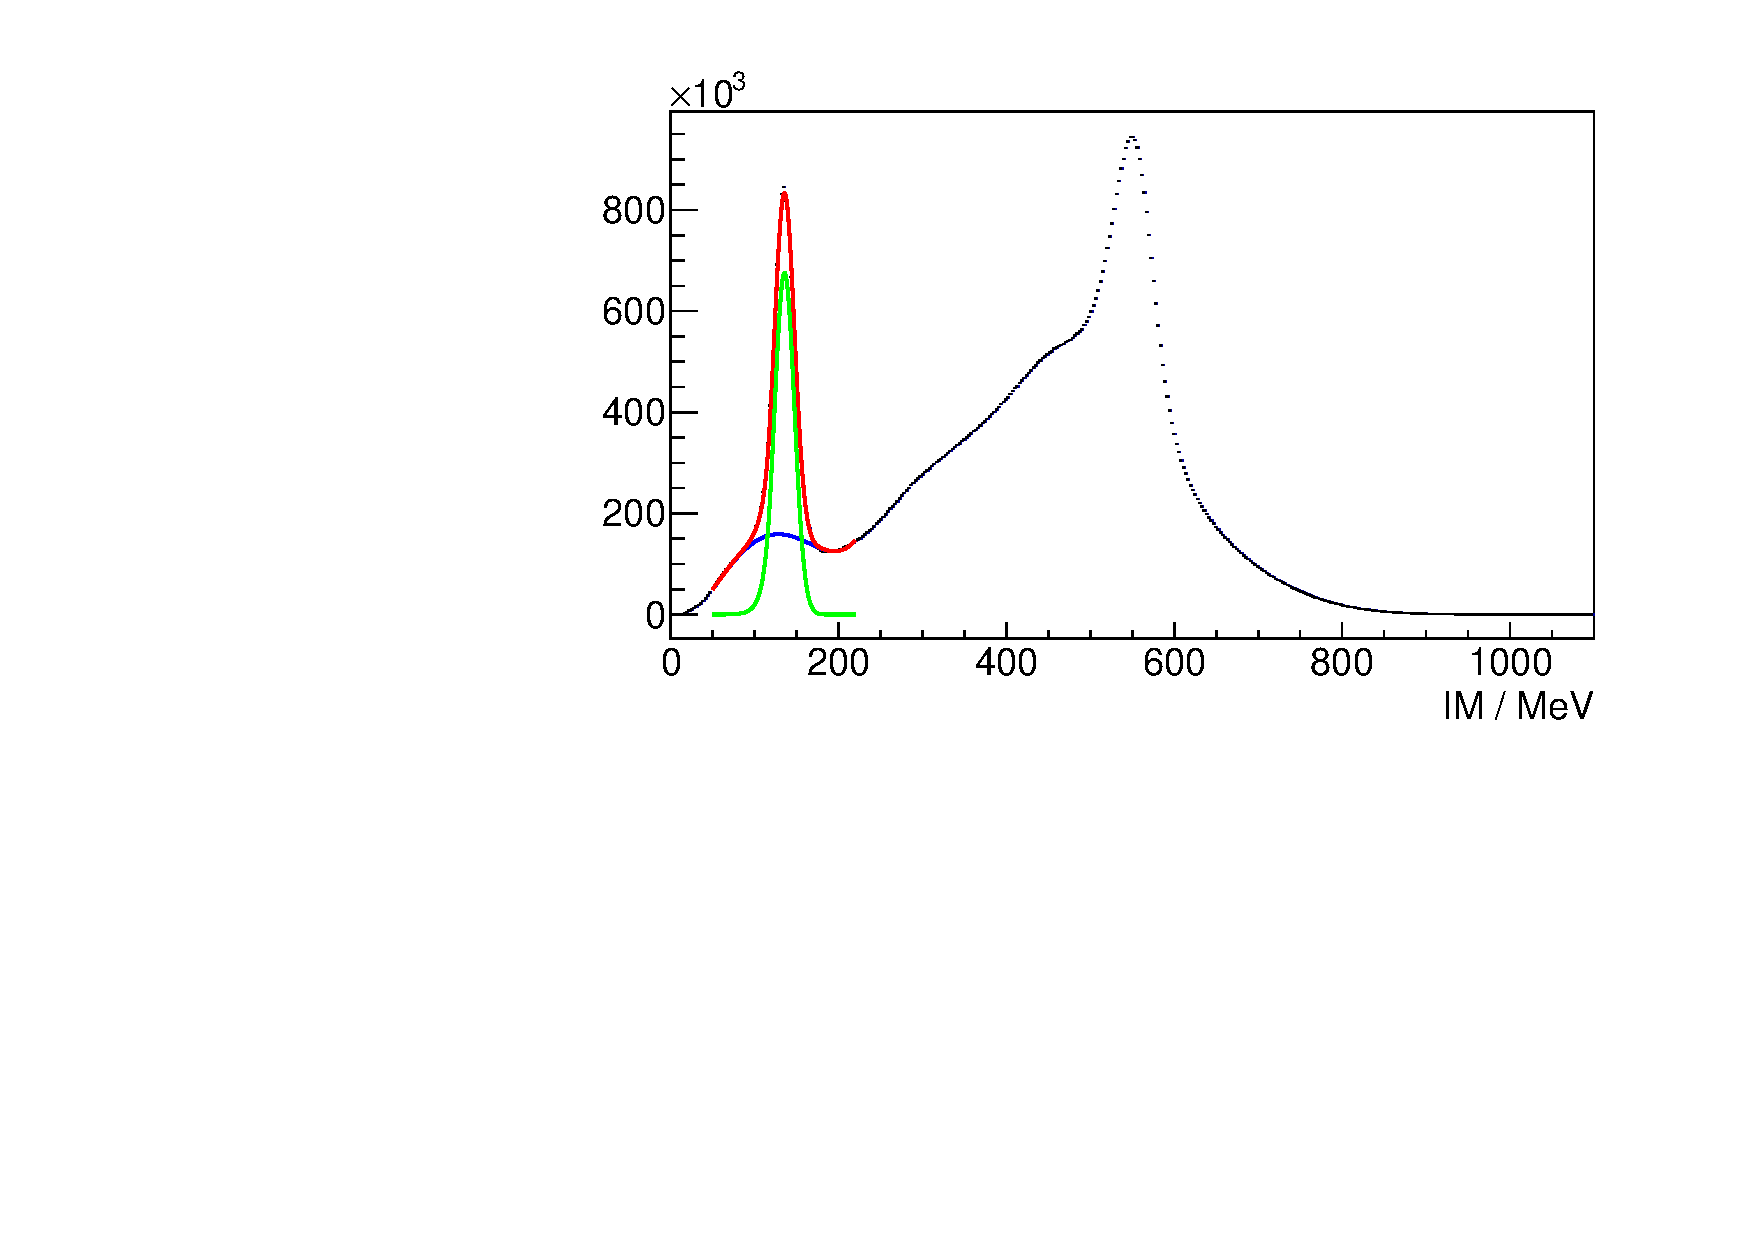
\includegraphics[width=0.50\textwidth]{Pictures/20171904RealIntervalFitExample}
	\hfill
		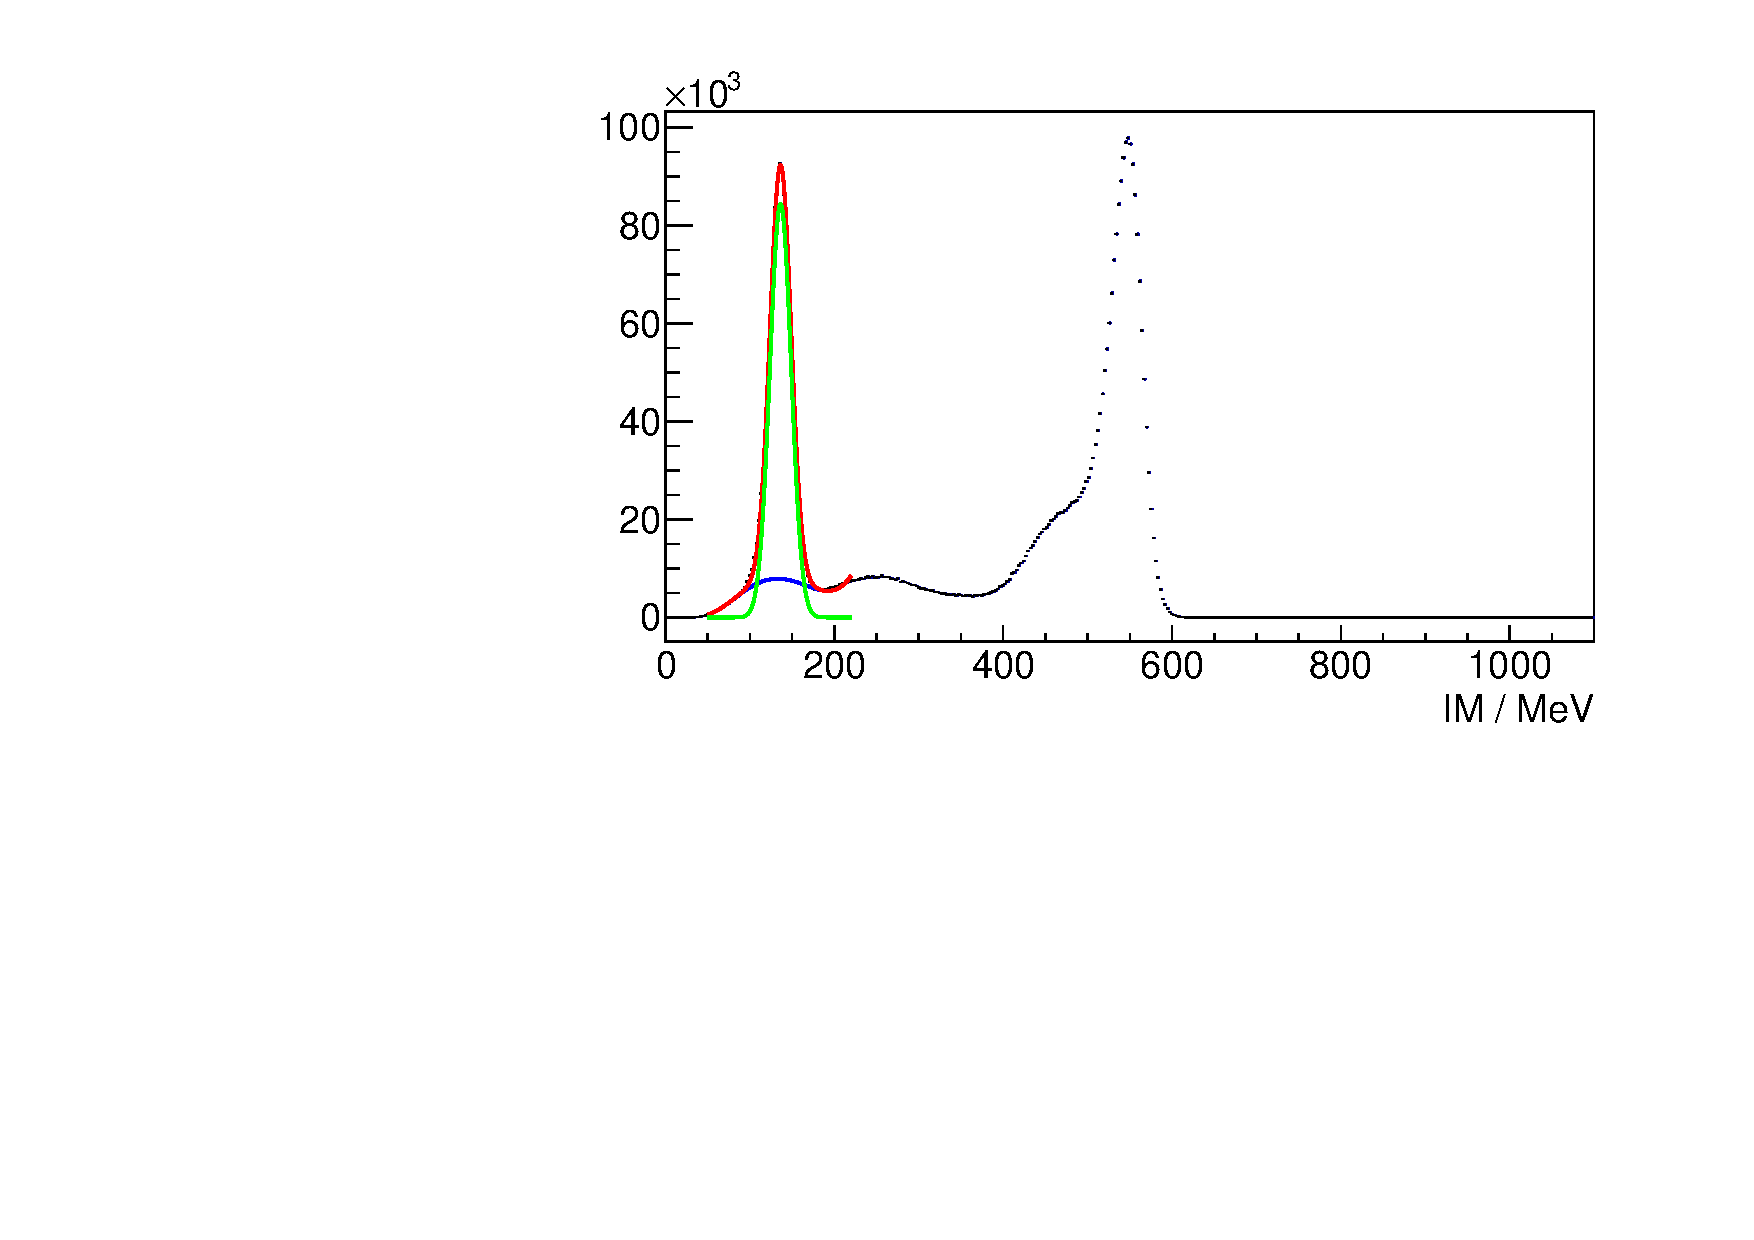
\includegraphics[width=0.50\textwidth]{Pictures/20171904RealUnchargedFitExample}
		
\end{figure}
\begin{tikzpicture}[remember picture,overlay]   
\coordinate (b) at (5.0 , 3.5);
\coordinate (c) at (5.7 , 3.5);
\draw [thick,black, ->,thick] (b) -- (c);
\end{tikzpicture}

\end{frame}
\begin{frame}
\frametitle{Event-Generator}


\begin{itemize}
	\item $|E_1 - E_2| < 25\,\text{MeV}$ is a strong cut. One need really large MC statistics. 
	
	$\rightarrow$ There is no MC sample with enough events
	\pause
	
	\item Creating a new sample with enough events with an already existing Event-Generator would take too much time (multiple days on blaster).
	Not Efficient!
	\pause
	
	\item It is better to use the same generator in all studies
	
	$\rightarrow$ The generator should be able to simulate MAMI-Beam and isotropic boost
\end{itemize}
\end{frame}

\begin{frame}
	\frametitle{Event-Generator in ANT}
	New Event-Generator integrated in ANT
	\begin{figure}
		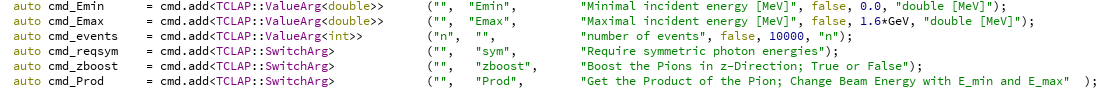
\includegraphics[width=1.1\textwidth]{Pictures/Gun}
		
	\end{figure}
	\begin{itemize}
		\item Emin: Minimal energy of the beam/boost
		\item Emax: Maximal energy of the beam/boost
		\item Events: Number of events
		\item Sym: Require $|E_{1}-E_{2}|<25\,\text{MeV}$
		\item ZBoost: Boost the $\pi^0$ in $z$-Direction, if false than isotropic boost
		\item Prod: Also takes the proton into account
	\end{itemize}
\end{frame}

\section{Studies}


\begin{frame}
	\frametitle{First look at real data}
	
	\begin{itemize}
		\item Beamtime October 2014
		\item Well-calibrated 
\end{itemize}
	
		\begin{figure}
		
		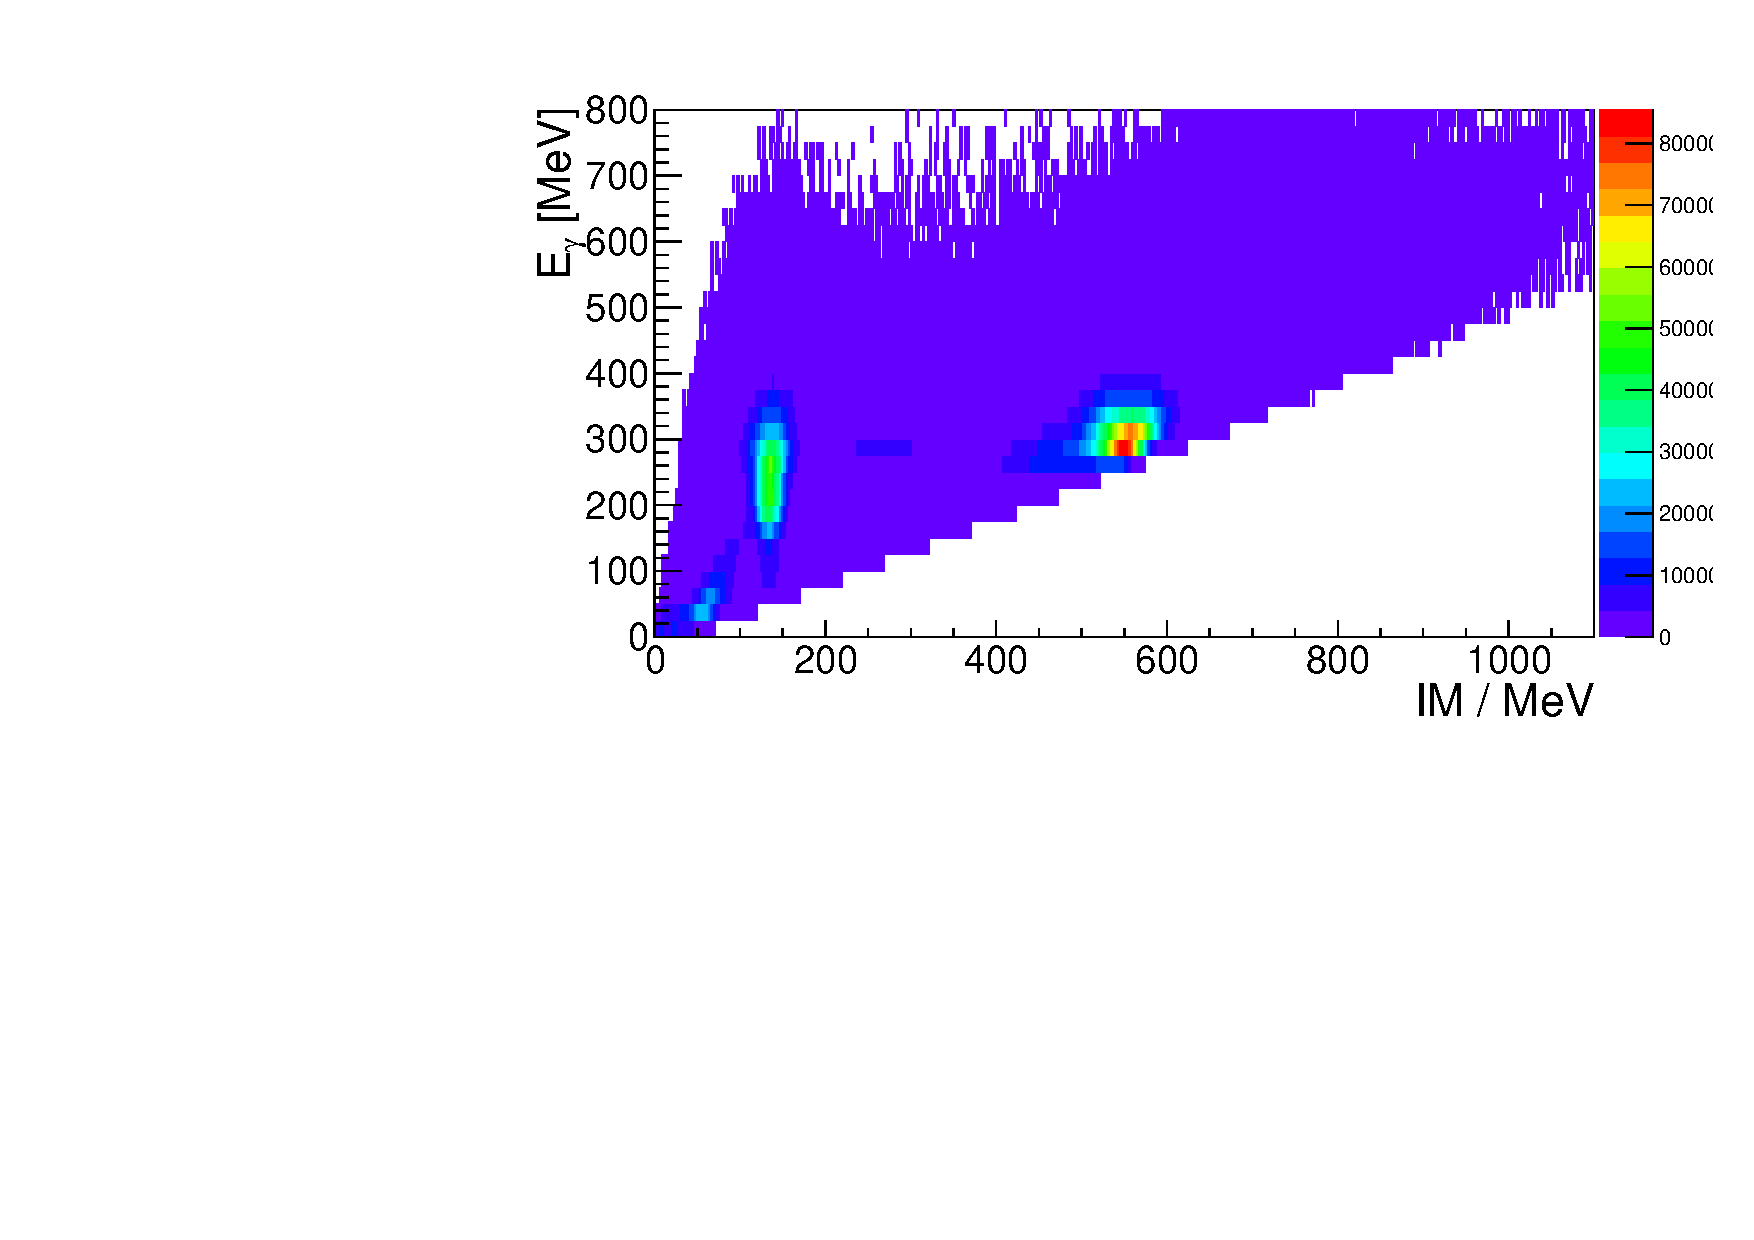
\includegraphics[width=0.50\textwidth]{Pictures/20171904Uncharged2DHist}
		\hfill
		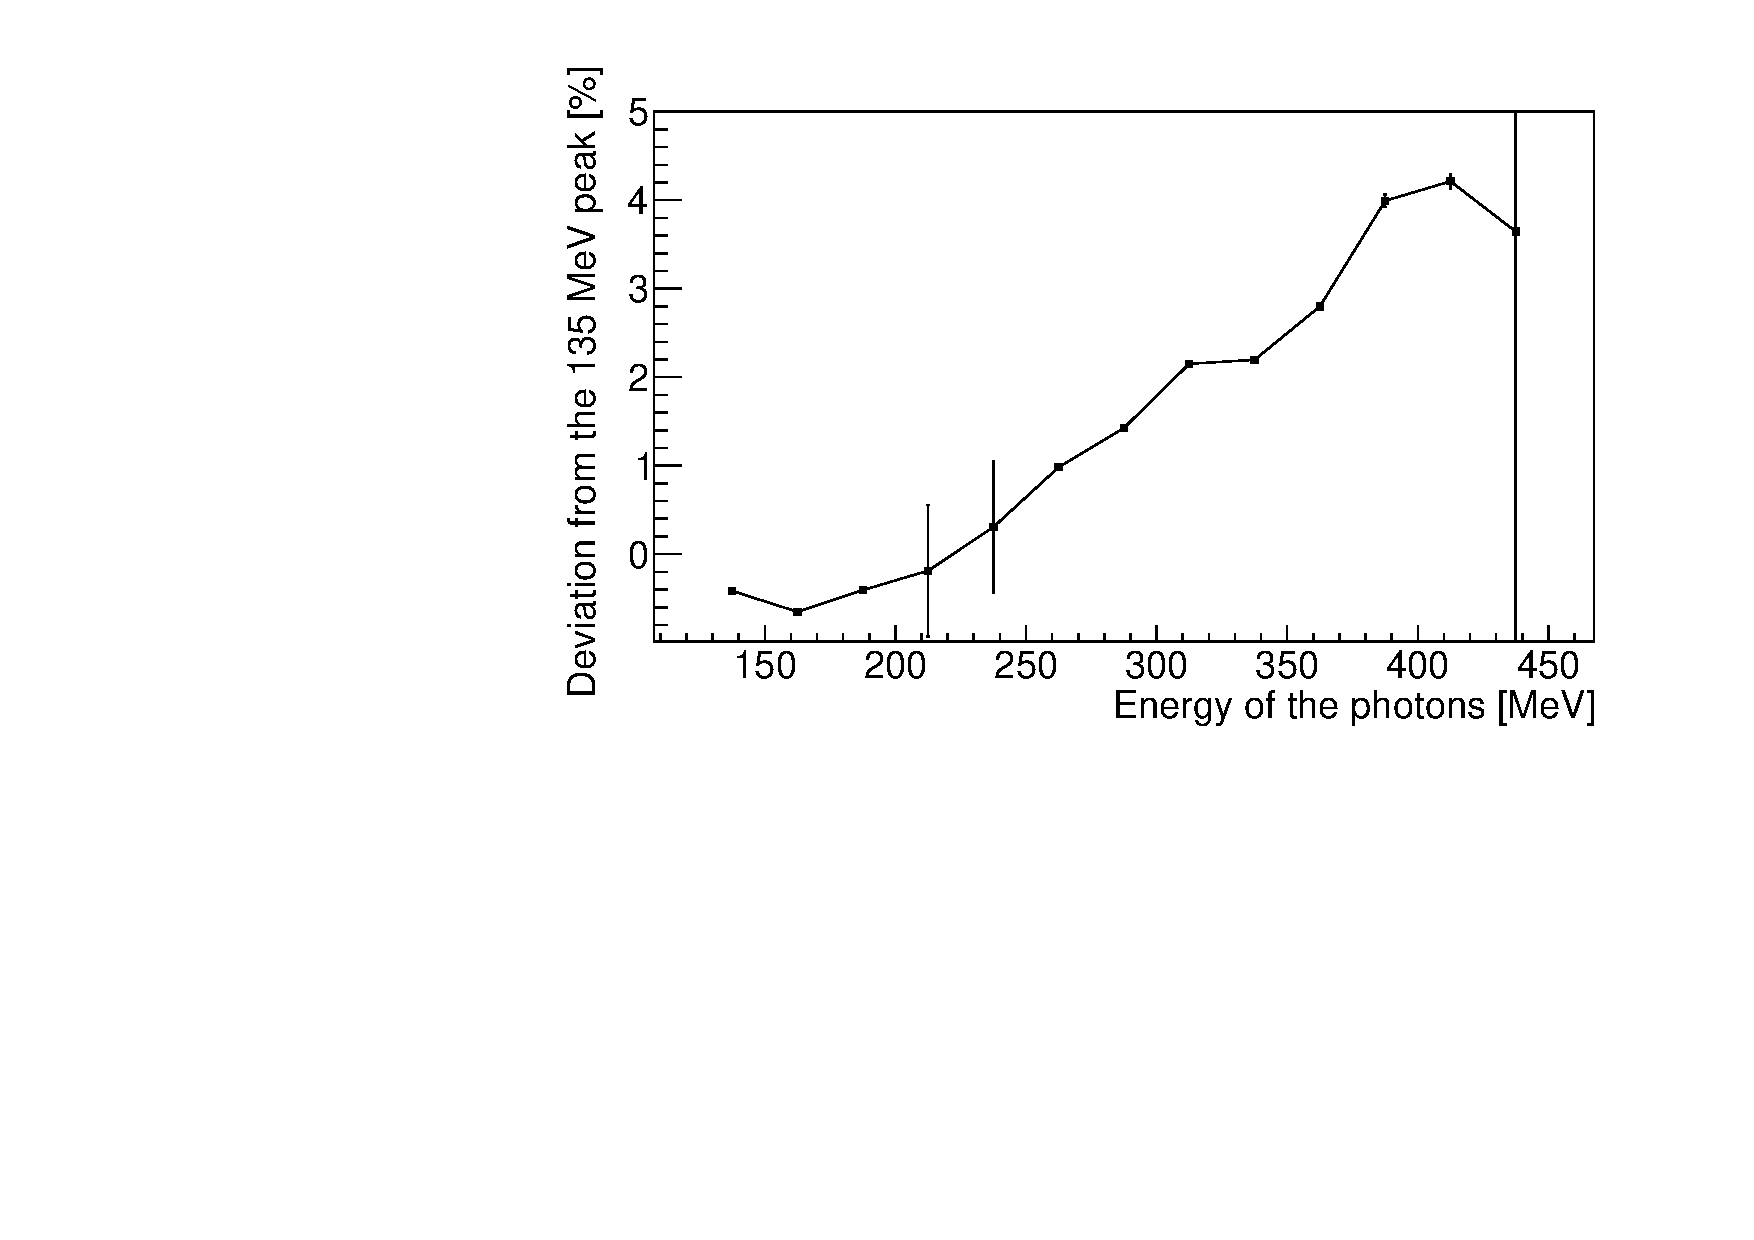
\includegraphics[width=0.50\textwidth]{Pictures/20170405StrahlzeitDeviatoinNoCut}
		
	\end{figure}
$\rightarrow$ There is a dependency	
\end{frame}

\begin{frame}
	\frametitle{Detectors on the Edge}
	
	\begin{itemize}
		\item Beamtime October 2014
		\item Neglect the detectors at the edge: They are difficult to calibrate because they have less neighbors
	\end{itemize}

\begin{figure}
	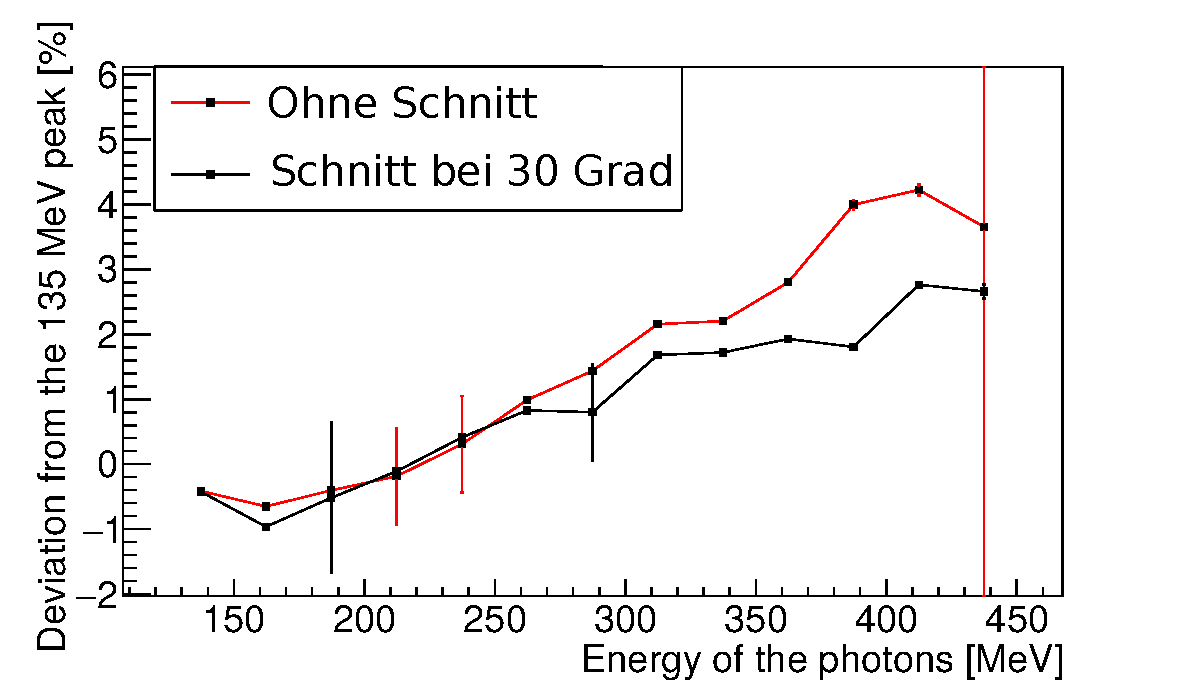
\includegraphics[width=0.75\textwidth]{Pictures/20170405StrahlzeitBothDeviation}
\end{figure}
	
\end{frame}

\begin{frame}
	\frametitle{How does MC look like?}
	\begin{itemize}
	
	
	\item Red:\, \, No additional cut
	
	Black: Neglect the detectors on the edge
		
	\end{itemize}

\begin{figure}
	
	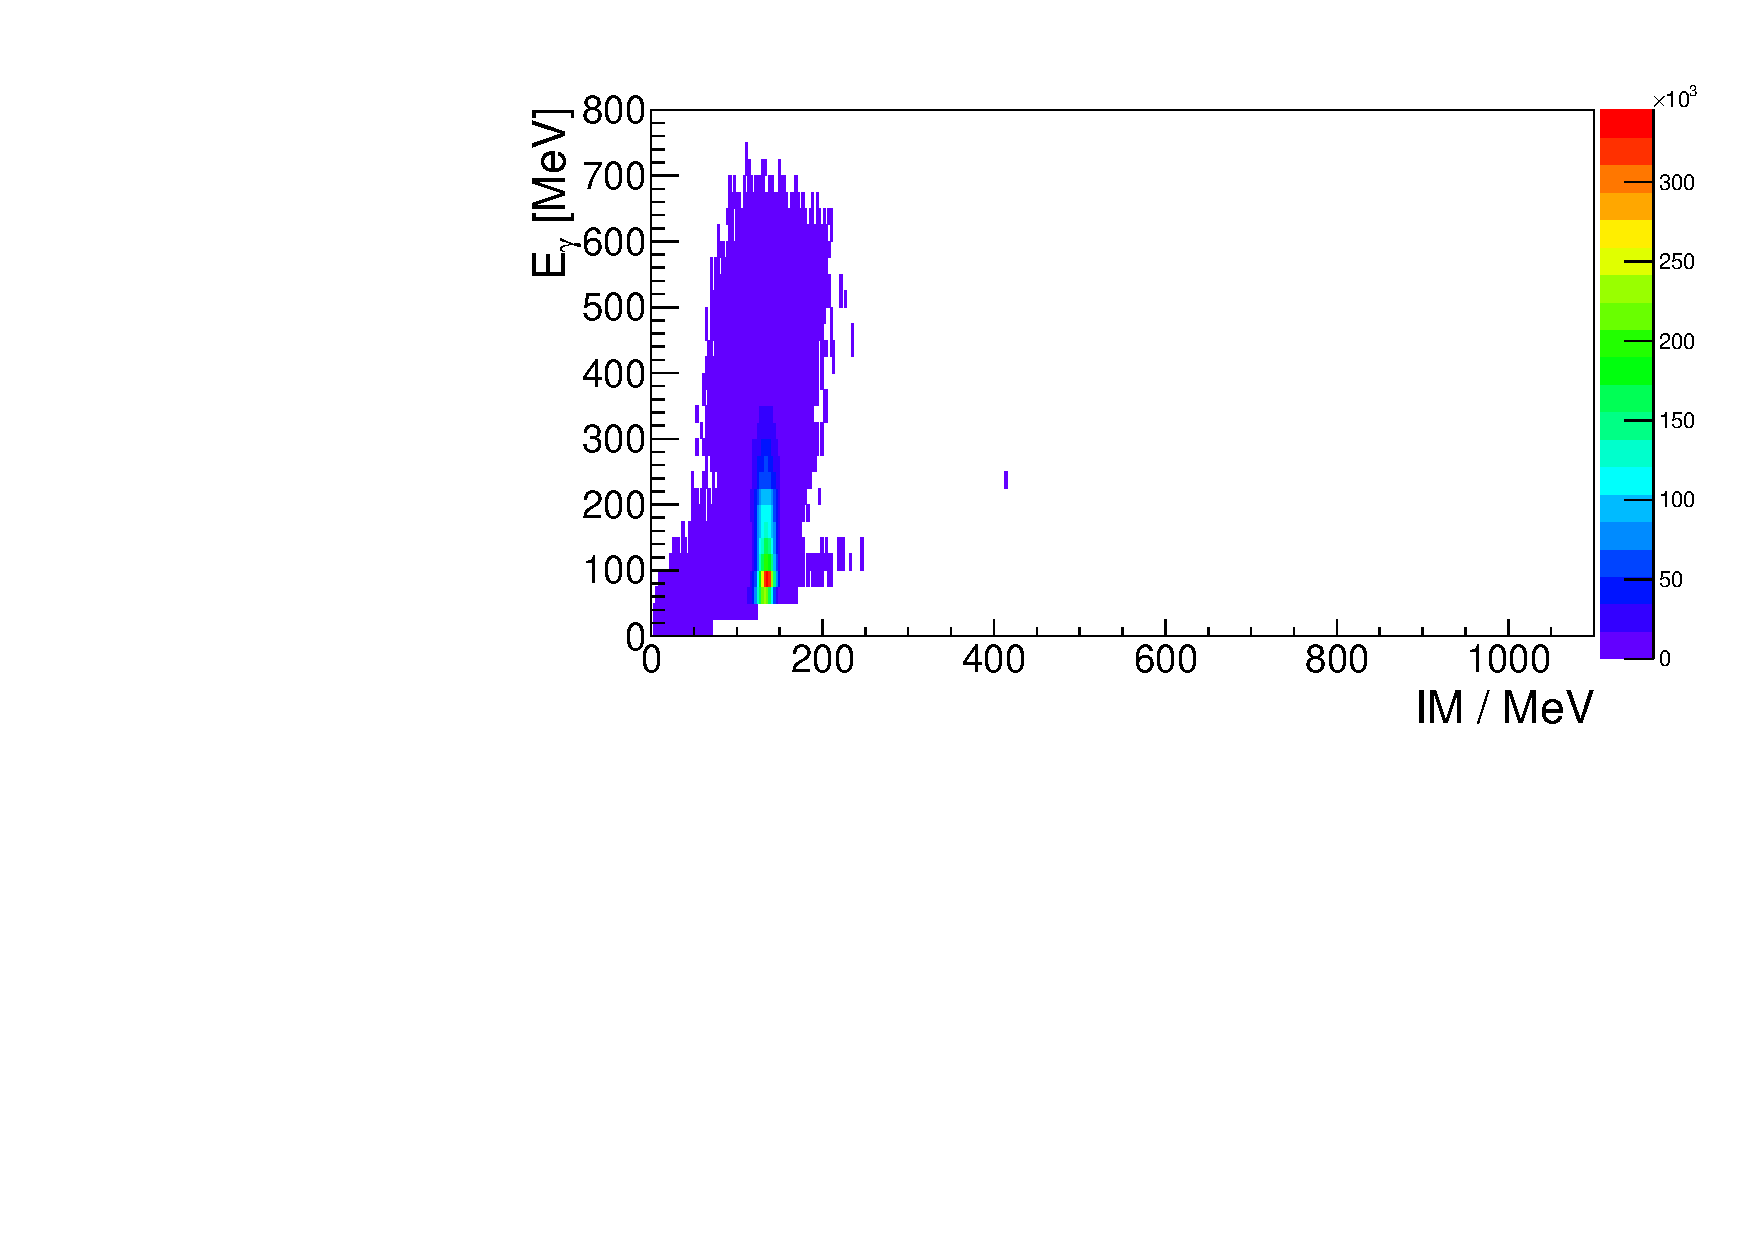
\includegraphics[width=0.50\textwidth]{Pictures/20171904SimNoCut2DHist}
	\hfill
	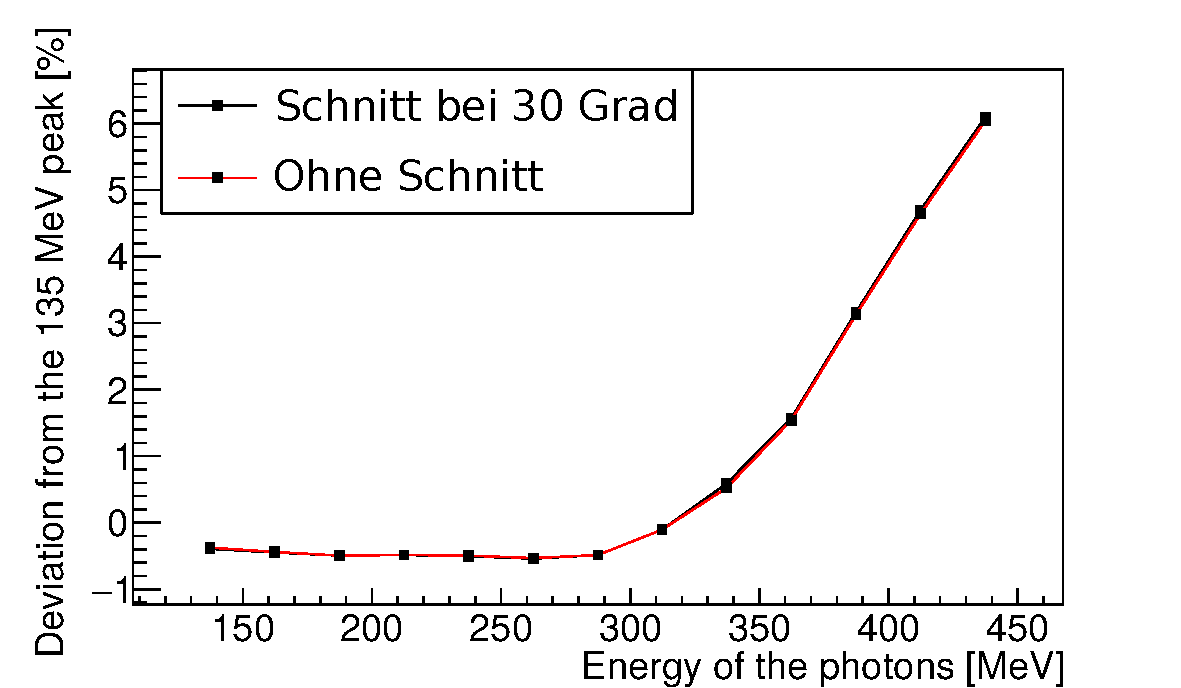
\includegraphics[width=0.50\textwidth]{Pictures/20172804MCBothDeviation}

\end{figure}	
	MC also shows this raise
	
	$\rightarrow$ it can be used for further studies
\end{frame}


\begin{frame}
	\frametitle{Isotropic Boost}
	\begin{itemize}
		\item $\pi^0$ decay in the origin of the target
		\item $\pi^0$ are boosted with an energy of $ 1420\, \text{MeV}$ to $1580\, \text{MeV}$ isotropically
		
		$\rightarrow$ all detector elements are hit roughly equally 
	\end{itemize}
	
	\begin{figure}
		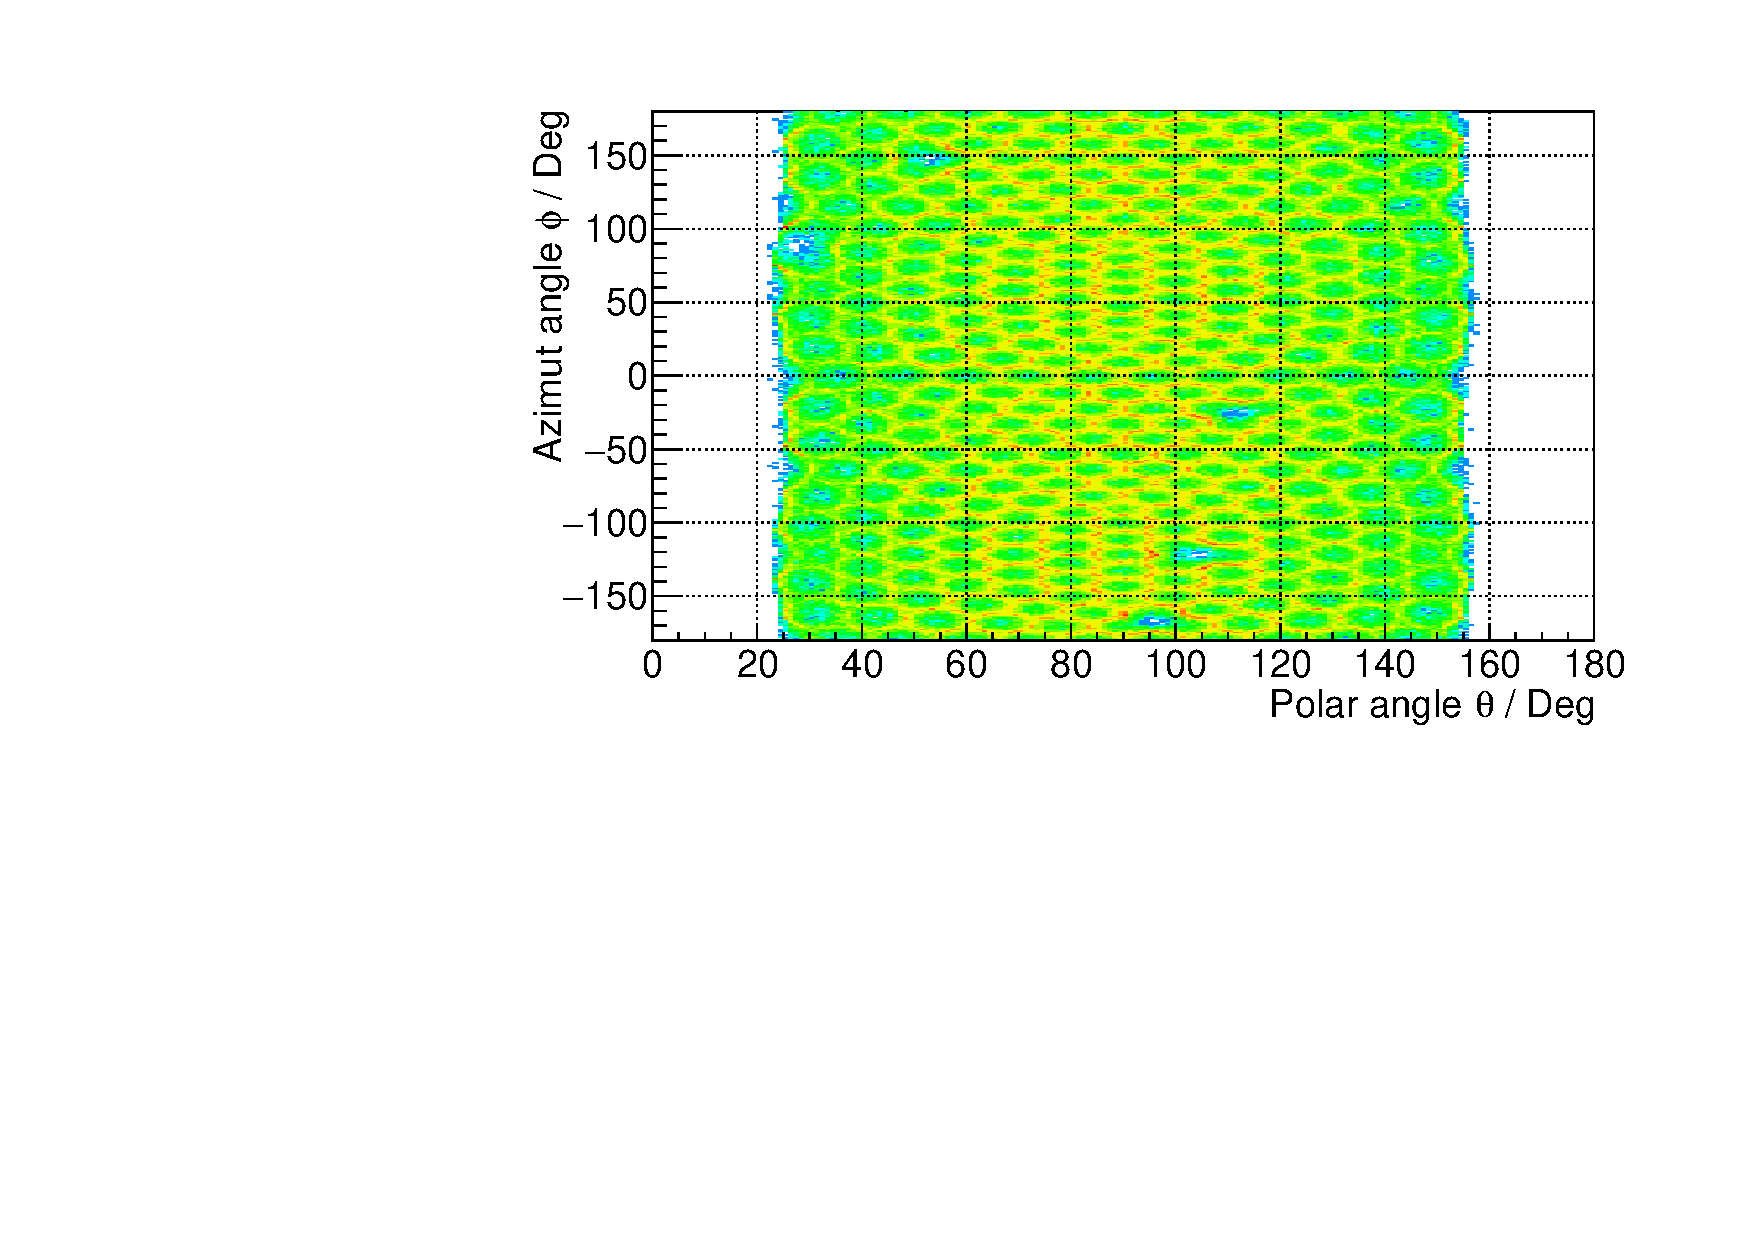
\includegraphics[width=0.50\textwidth]{Pictures/20171204DistributionPhotonUrsprungIsotrop}
		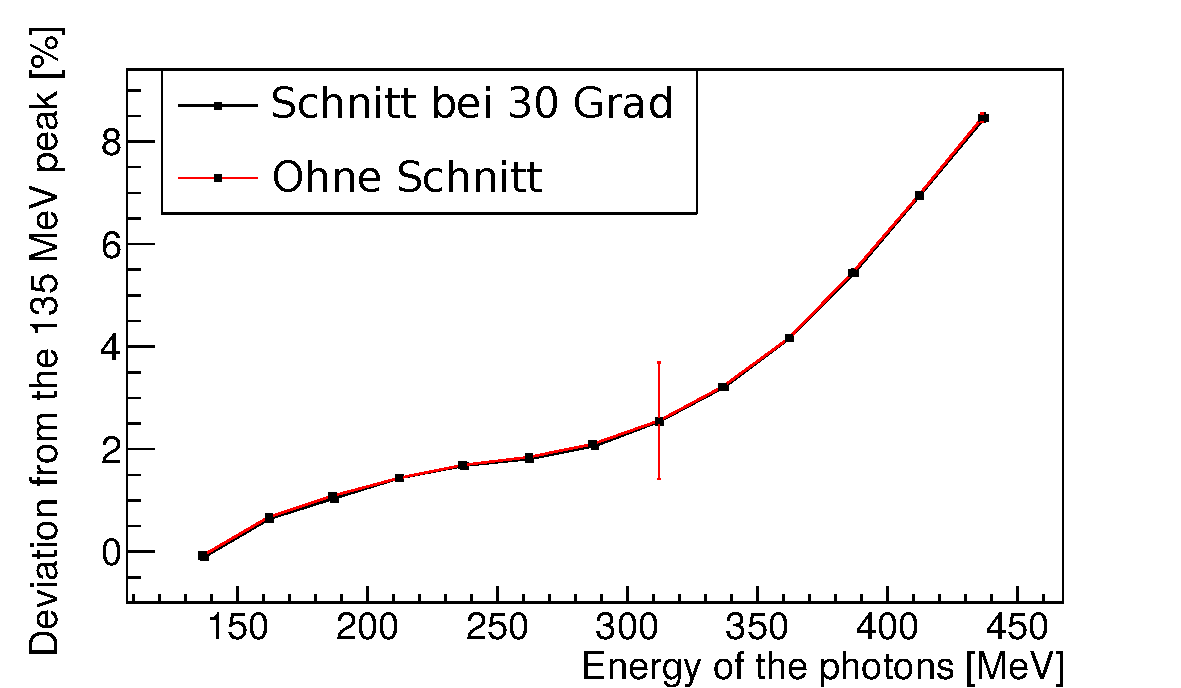
\includegraphics[width=0.50\textwidth]{Pictures/20172804IsotropUrpsprungDeviation}
	
	\end{figure}
$\rightarrow$ Raise is not caused by specific detector elements
\end{frame}

\begin{frame}
	\frametitle{Dimension of the Target}
	\begin{figure}
	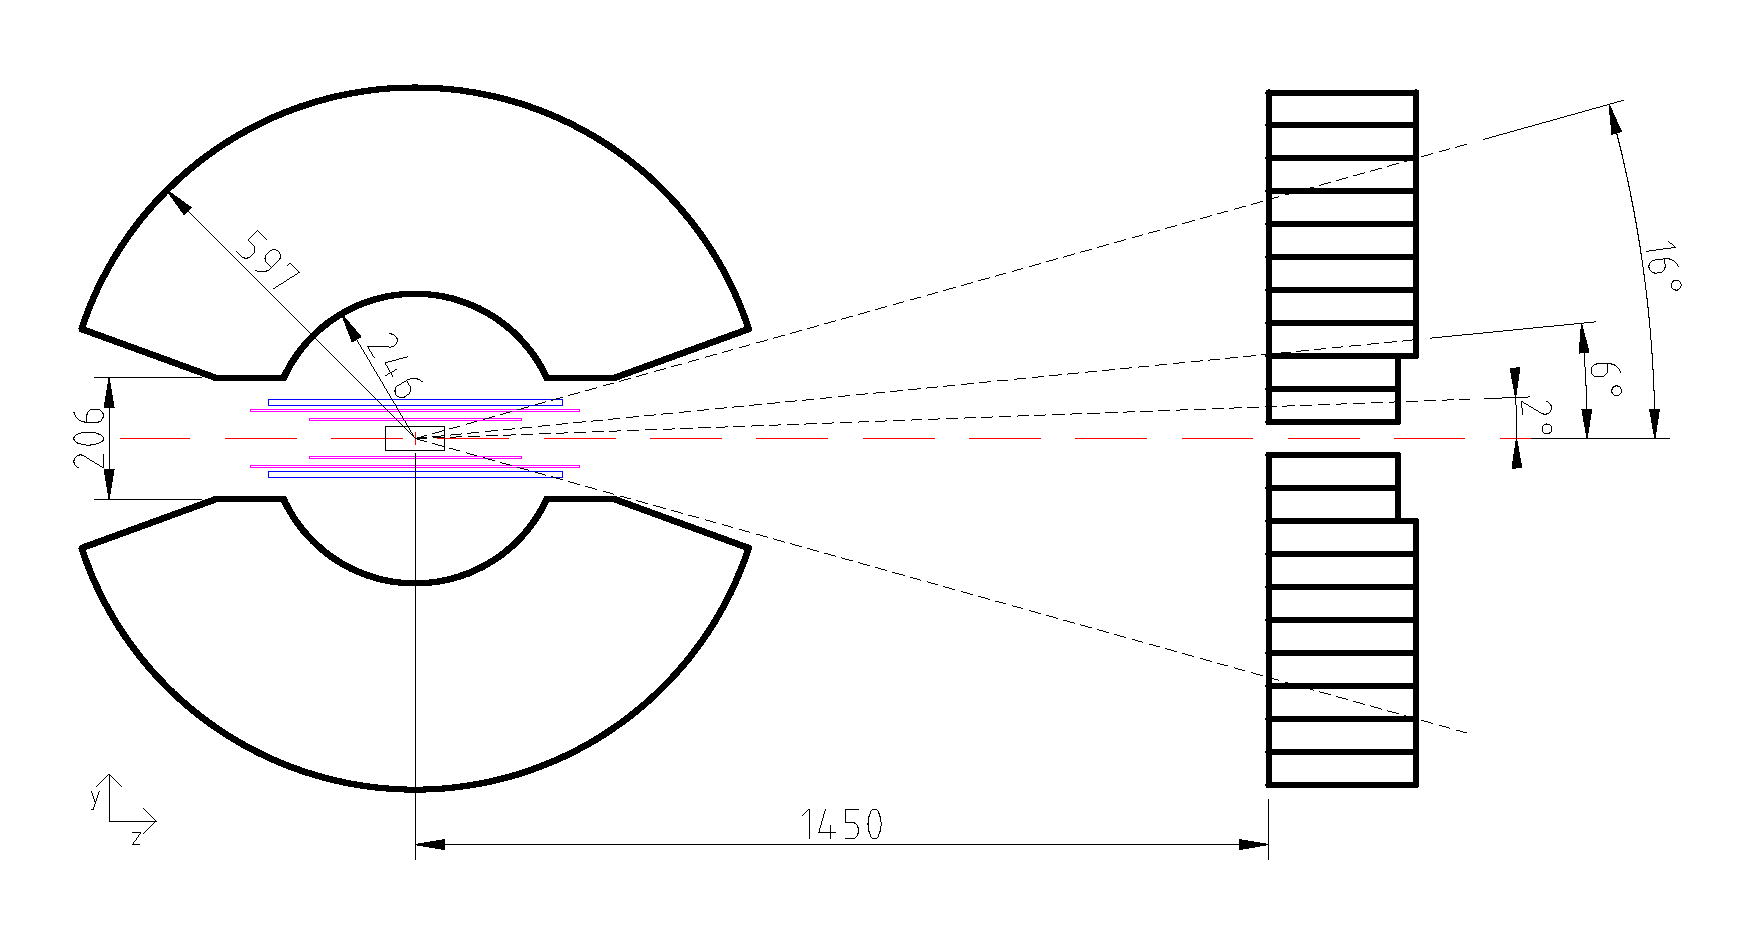
\includegraphics[width=1.00\textwidth]{Pictures/cbtaps_side.pdf}
	\end{figure}
	
	
\end{frame}


\begin{frame}
	\frametitle{$z$-Vertex Dependency}
	\begin{itemize}

		\item Neglect the detectors on the edge
		\item Divide the target in sections of $1\,\text{cm}$
	\end{itemize}


\begin{figure}
	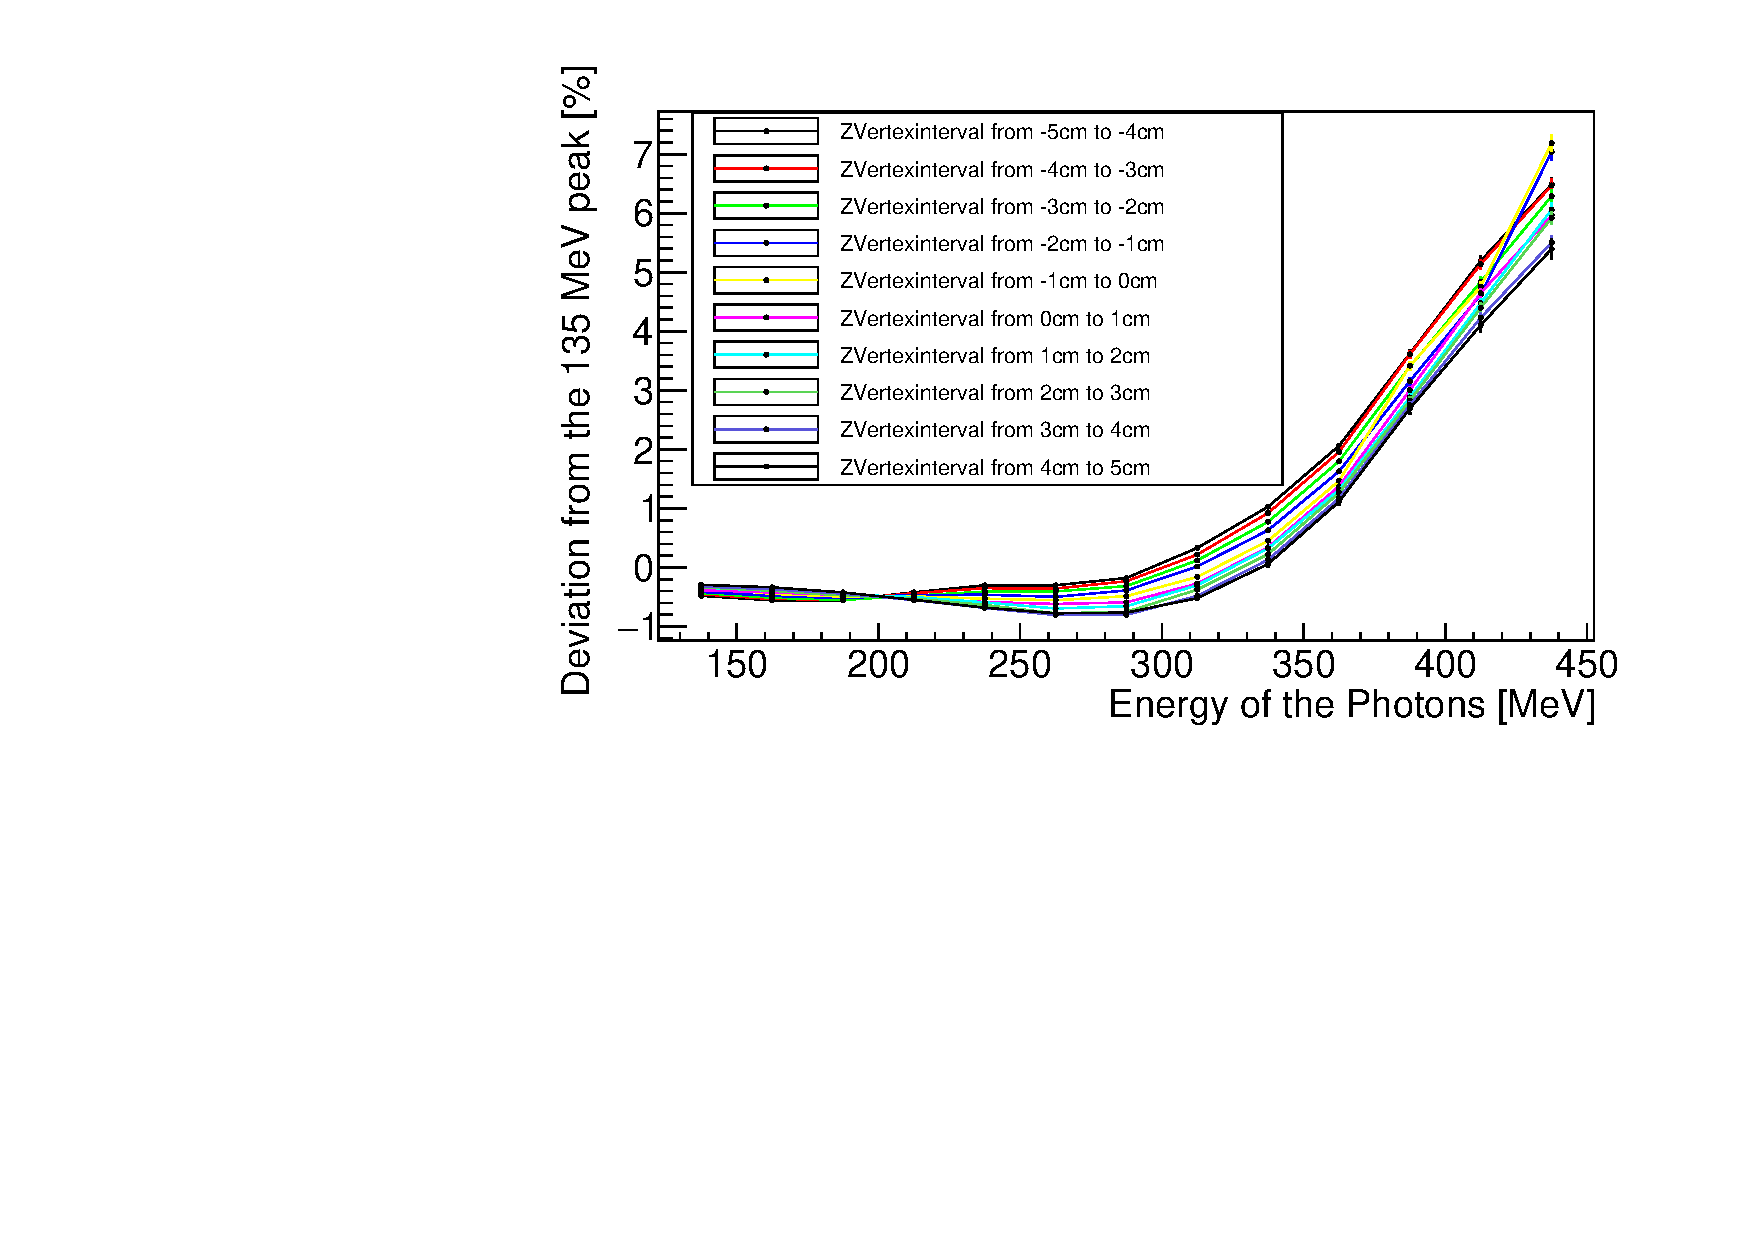
\includegraphics[width=0.750\textwidth]{Pictures/20172804MCZVertexDeviation}
	
\end{figure}
$\rightarrow$ Some dependence but small in compared to the main effect
\end{frame}

\begin{frame}
	\frametitle{Angle between Generated and Reconstructed Candidates }

\begin{itemize}

	\item The angle between generated and reconstructed candidate is calculated
\end{itemize}

\begin{figure}
	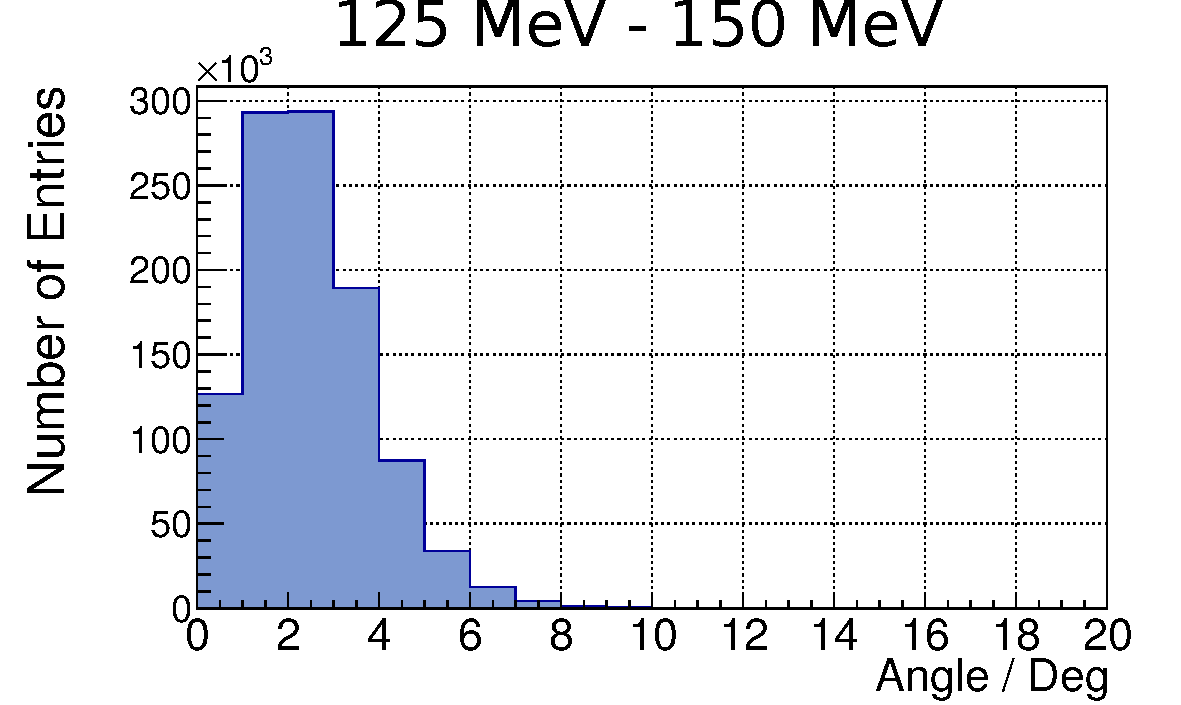
\includegraphics[width=0.5\textwidth]{Pictures/20172604AngleRegGen100-125MeV}
	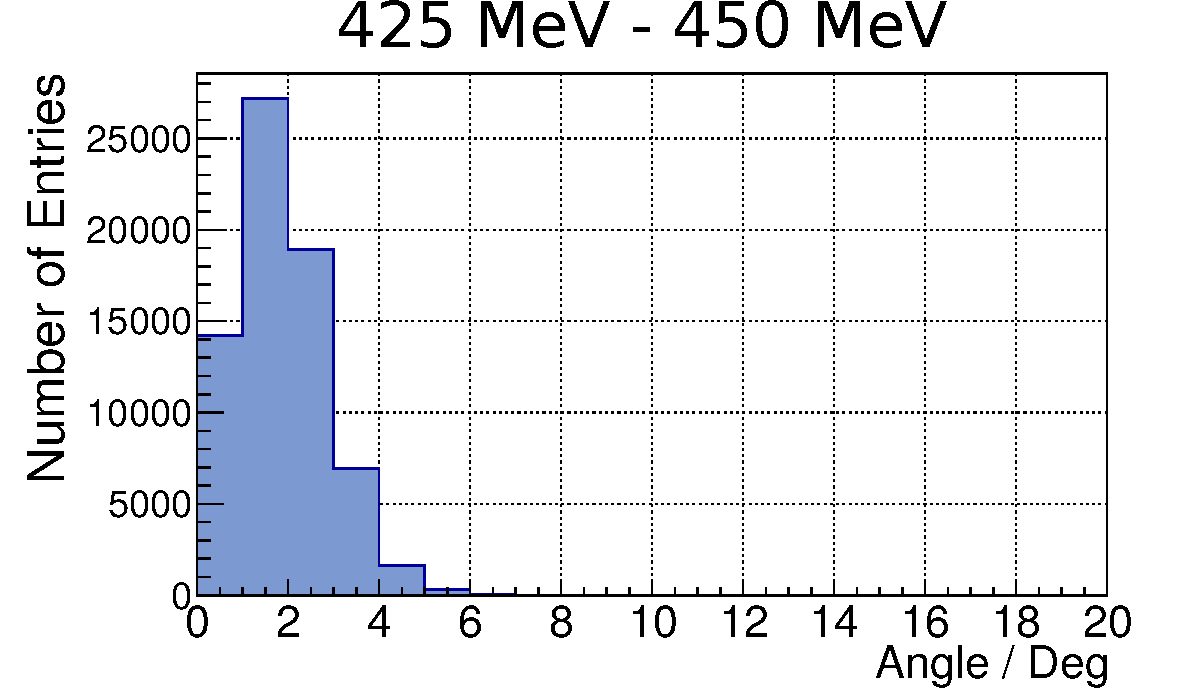
\includegraphics[width=0.5\textwidth]{Pictures/20172604AngleRegGen400-425MeV}

\end{figure}
$\rightarrow$ Angular resolution $\sim 1^{\circ} \,\text{to}\,2^{\circ}$

\end{frame}

\begin{frame}
	\frametitle{Difference between Generated and Reconstructed Opening Angle}
	
	\begin{itemize}
		\item $\Delta \alpha = \alpha_{rec}-\alpha_{gen}$
	\end{itemize}
\begin{figure}
	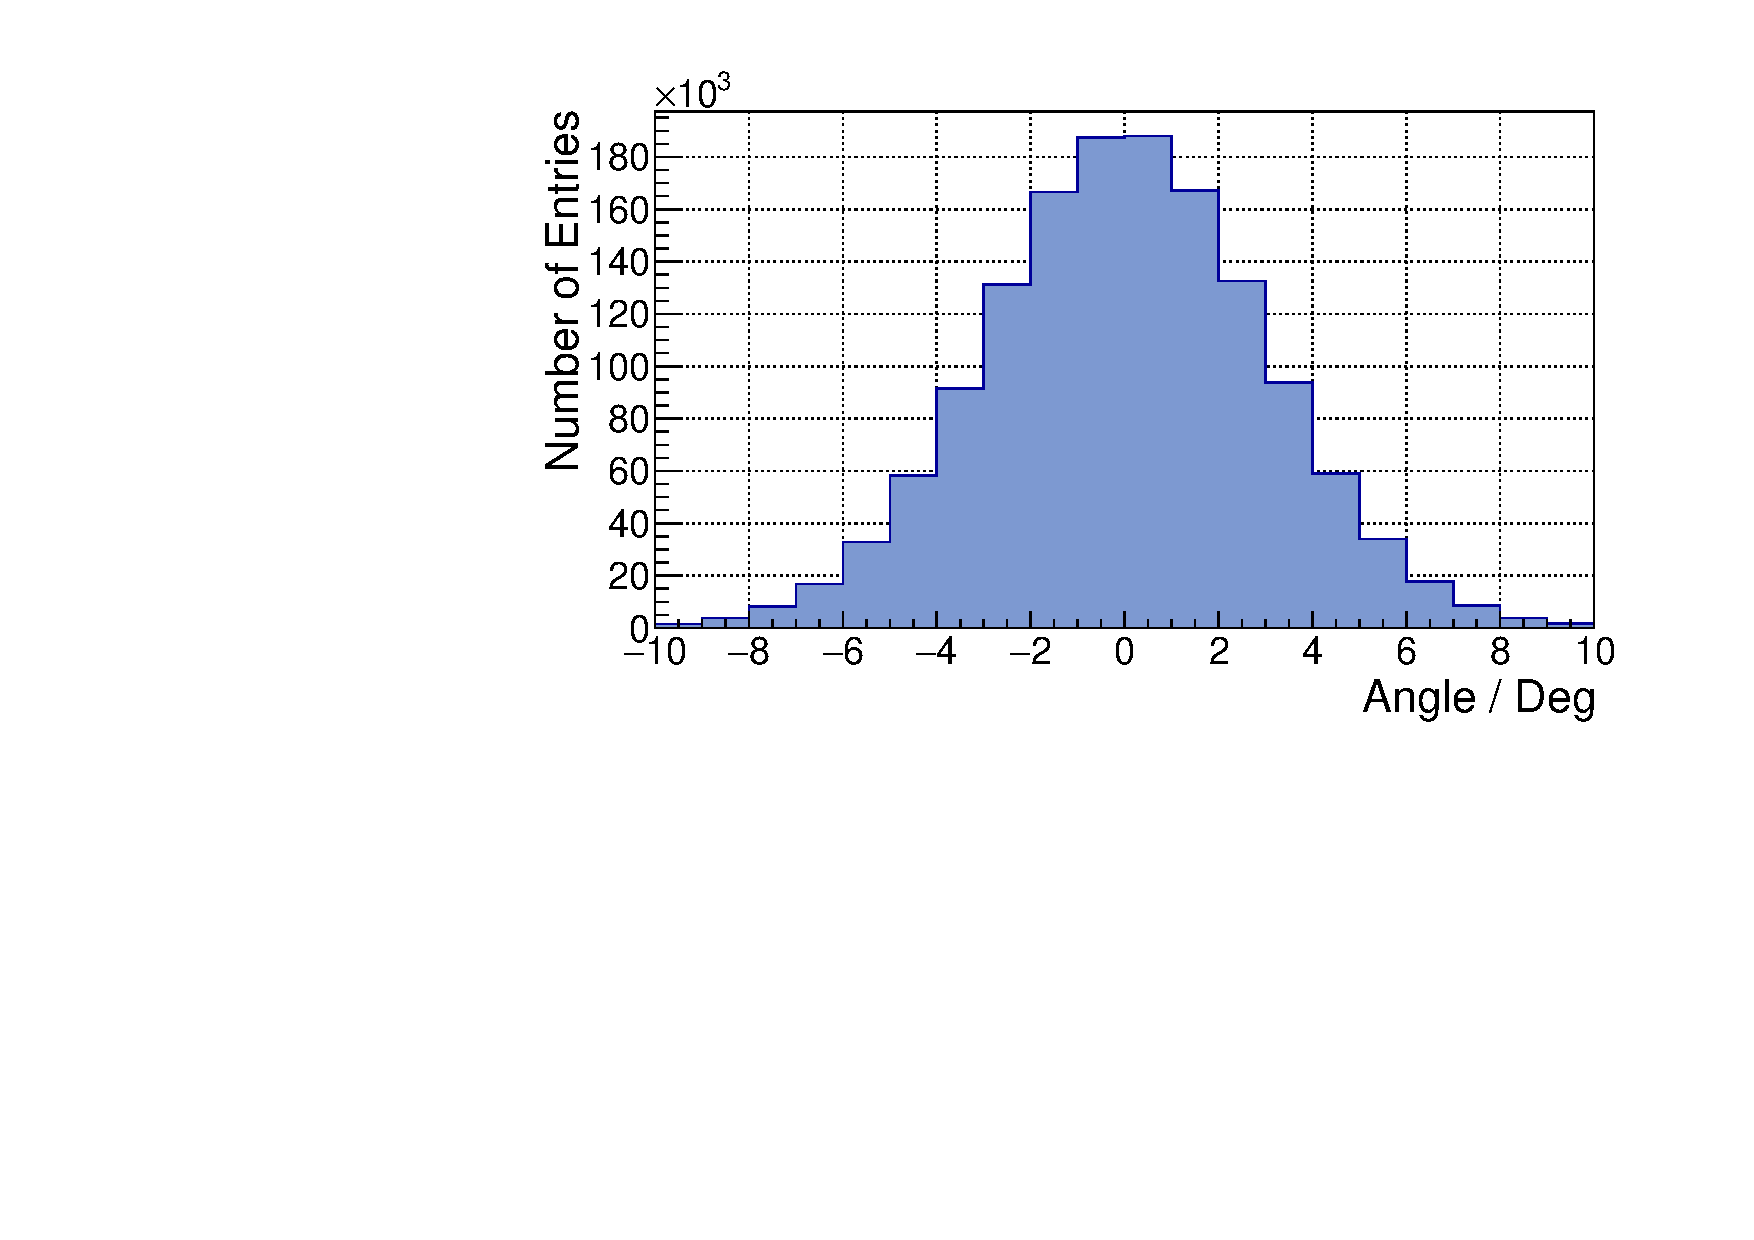
\includegraphics[width=0.5\textwidth]{Pictures/20172704MCDeviationOpeningAngle125MeV}
	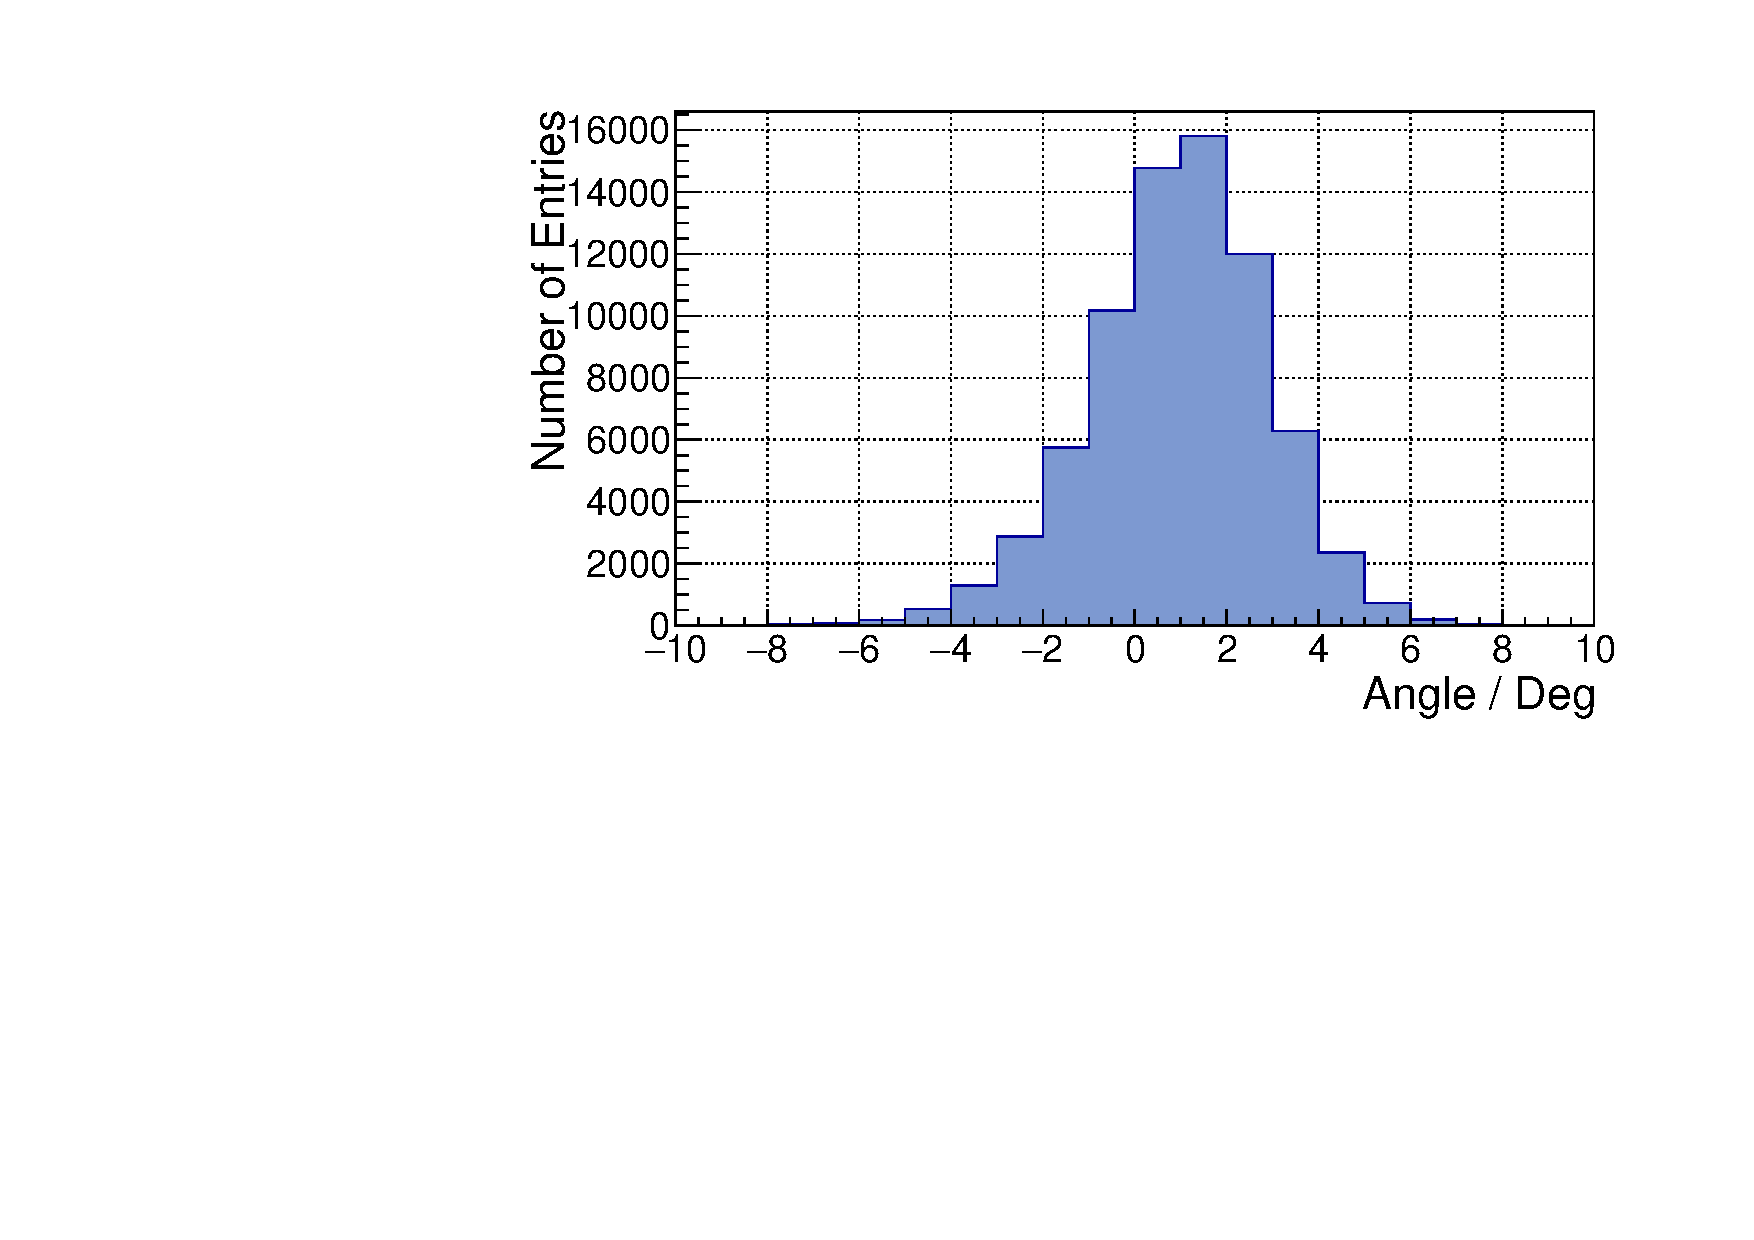
\includegraphics[width=0.5\textwidth]{Pictures/20172704MCDeviationOpeningAngle400MeV}

\end{figure}
$\rightarrow$ Systematic bias for high photon energies

\begin{picture}(5,1)

\put(120,135){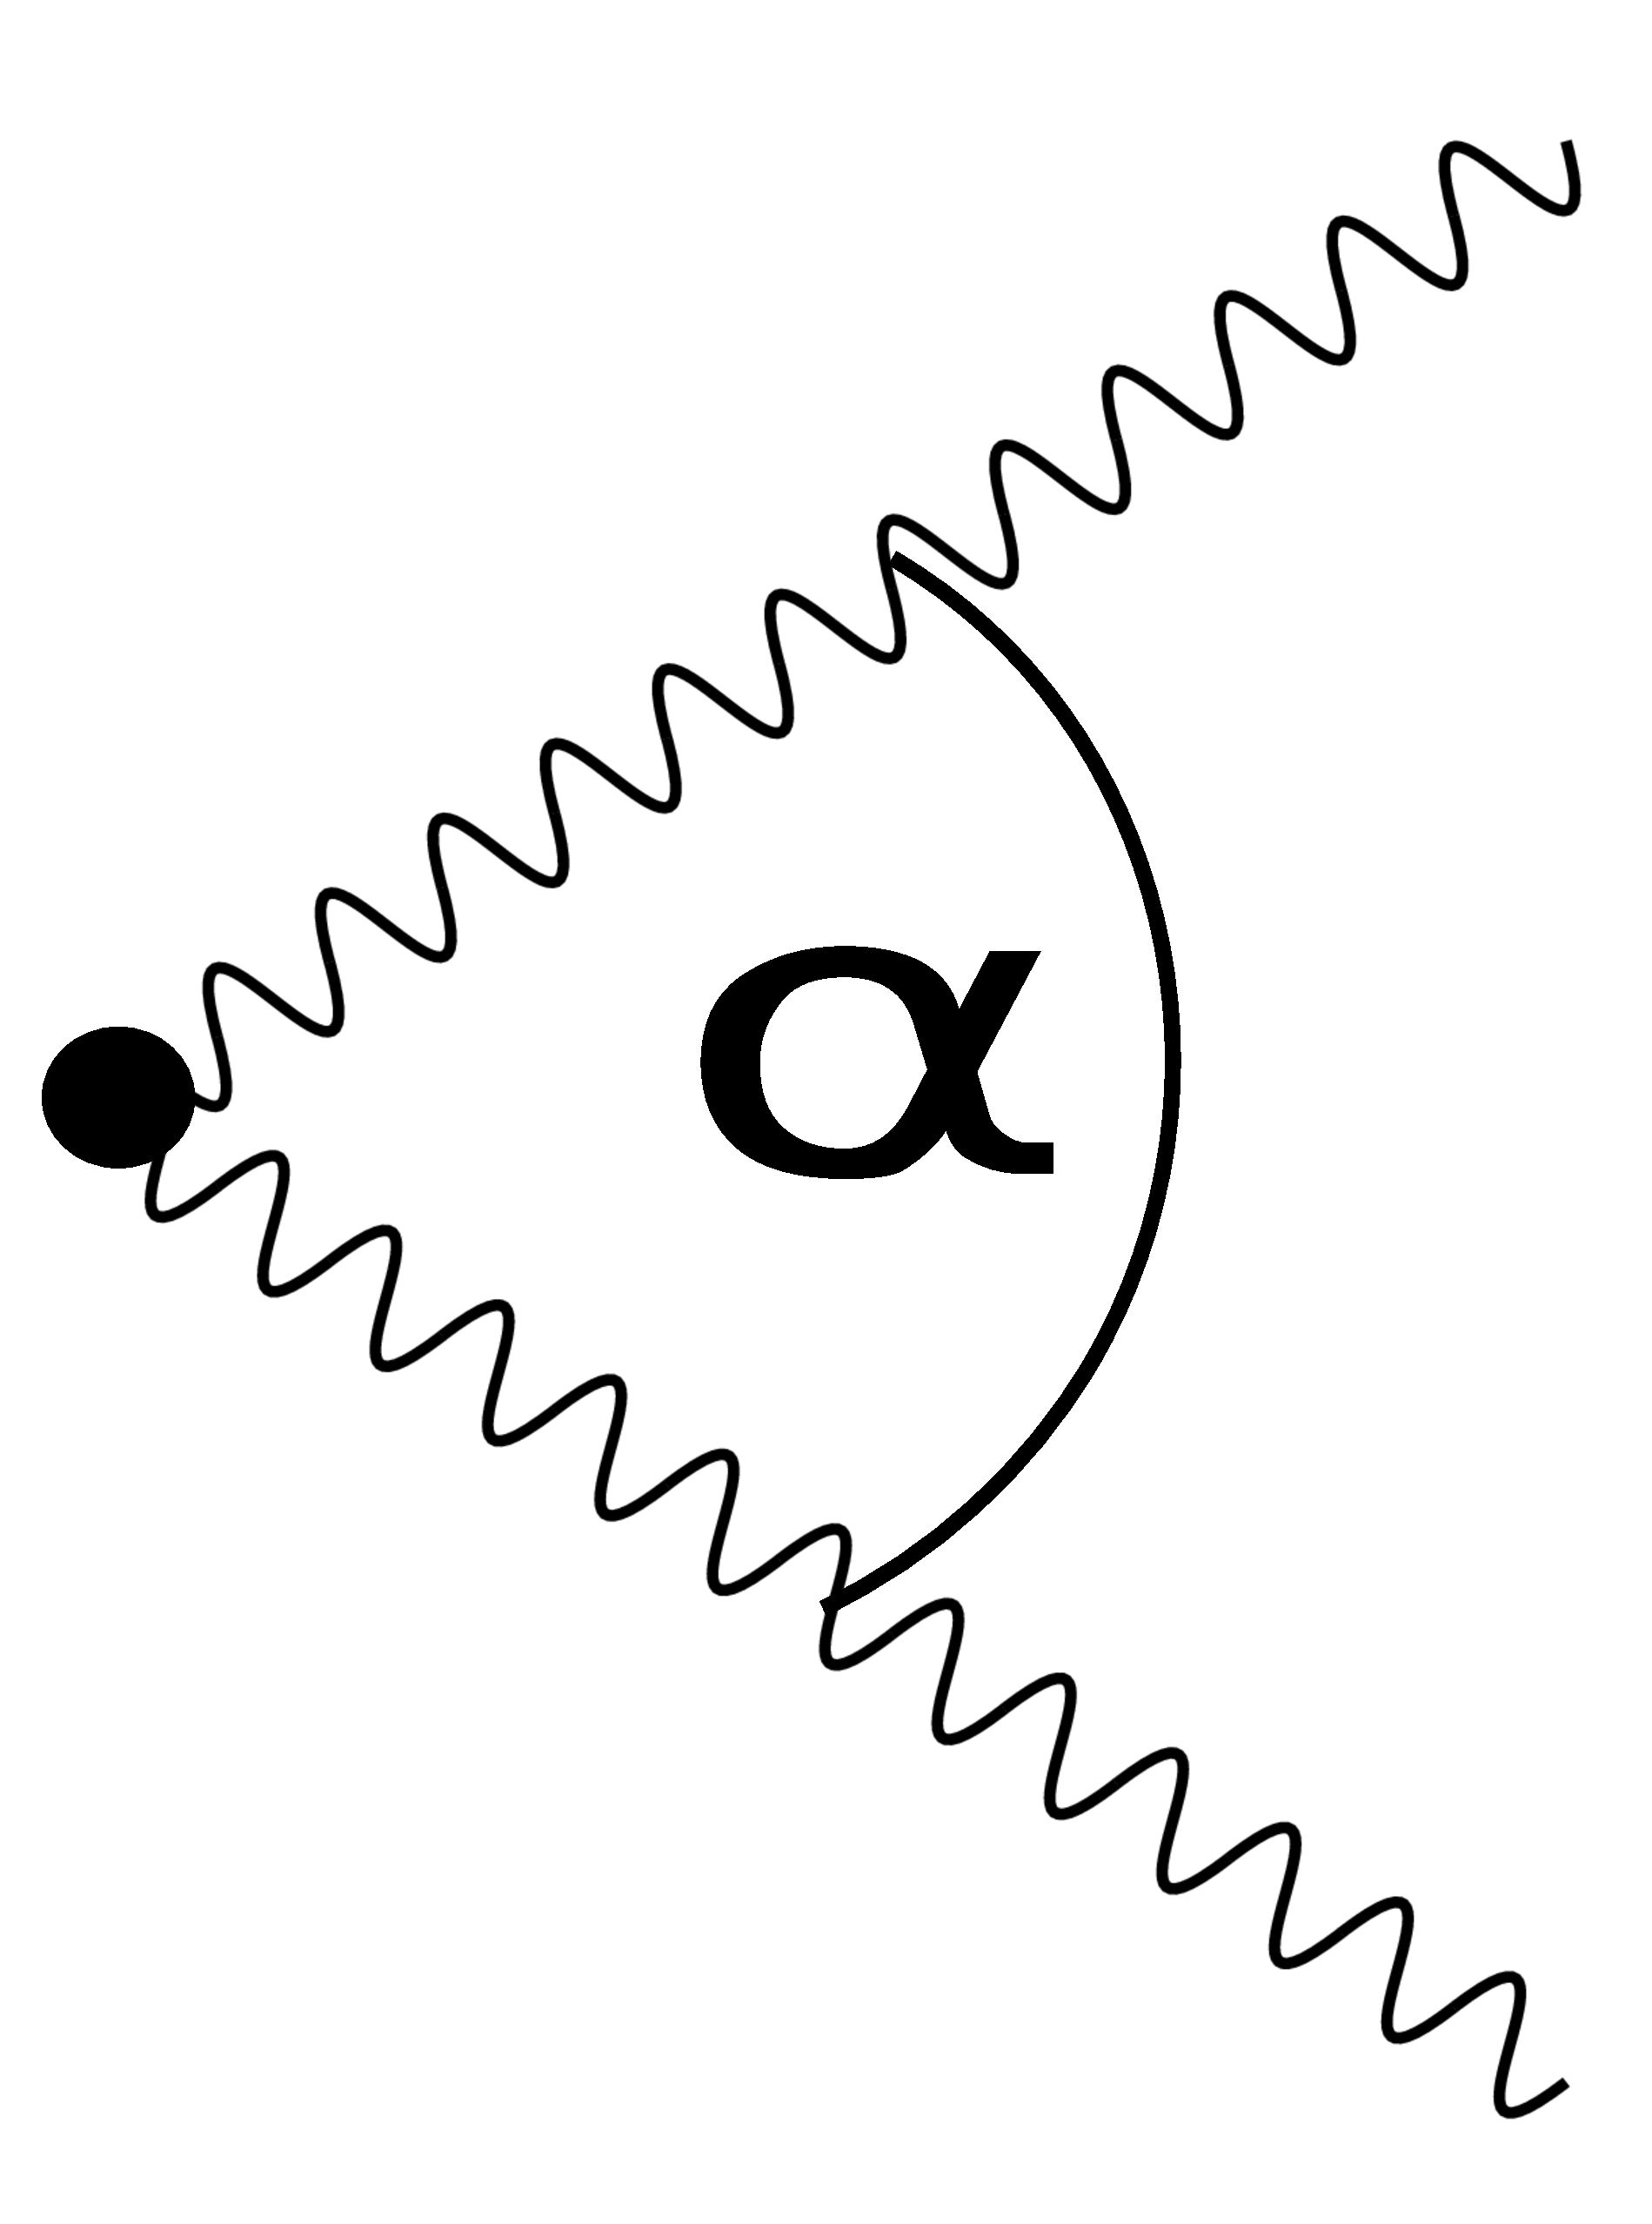
\includegraphics[width=0.1\textwidth]{Pictures/oangle.pdf}}

\end{picture}
\end{frame}

\begin{frame}
	\frametitle{Reason for the Deviation?}
	\begin{center}
	
	$m_{\pi^0}=\sqrt{2 E_1E_2(1-\text{cos}(\alpha))}$
	
		$\rightarrow \Delta m_{\pi^0} =\sqrt{E_1 E_2} \cdot \text{cos}(\frac{\alpha}{2}) \cdot \Delta \alpha$
		\end{center} 
		
			\begin{center}
				
		with $E_1 = E_2 = 450\,\text{MeV}$ $\rightarrow \alpha \approx  17.3^{\circ}$
		
	\end{center}
			
	\begin{center}
					
		Lets assume: $\Delta \alpha = 1.0^{\circ}$
		
		$\rightarrow \Delta m_{\pi^0} = 7.8\,\text{MeV}$
		
		Which is a deviation of about $6\%$ to the true $m_{\pi^0}$ mass
		
	\end{center}

\end{frame}


\begin{frame}
	\frametitle{$\Delta \alpha$ for Different $z$-Vertices}
	\begin{itemize}
		\item $\Delta \alpha$ for different $z$-Vertices
	\end{itemize}

\begin{figure}
	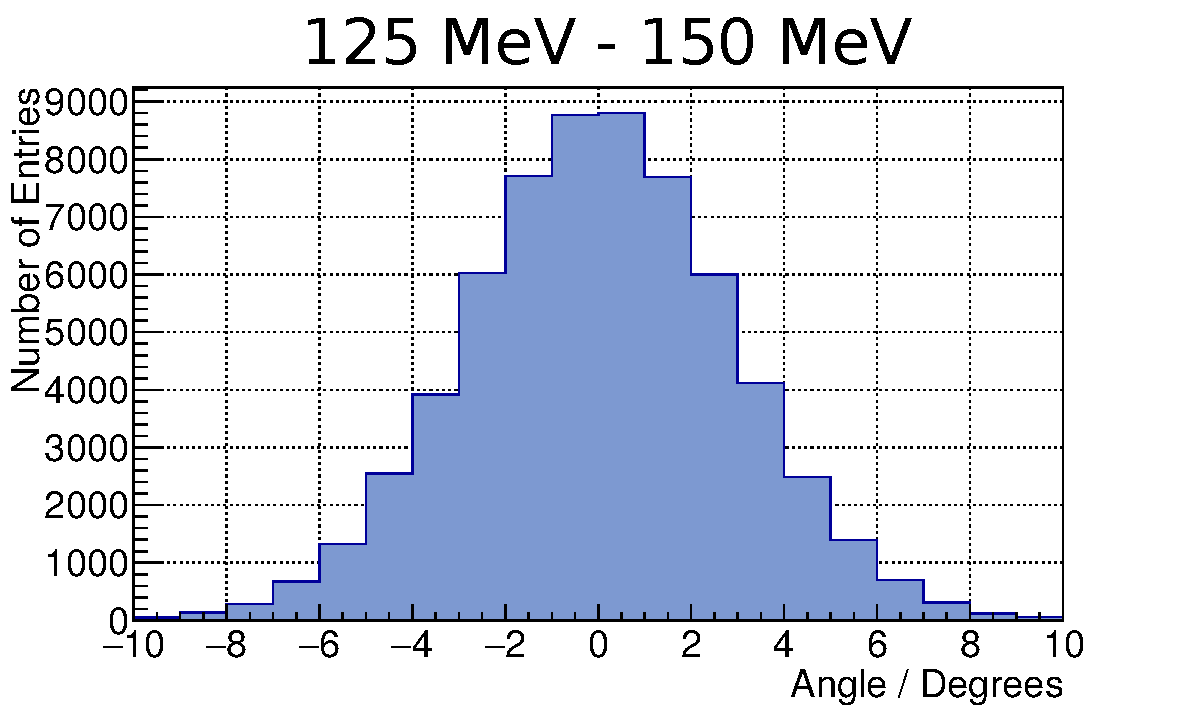
\includegraphics[width=0.35\textwidth]{Pictures/20170205DiffOeffZVertex-4_125MeV}
	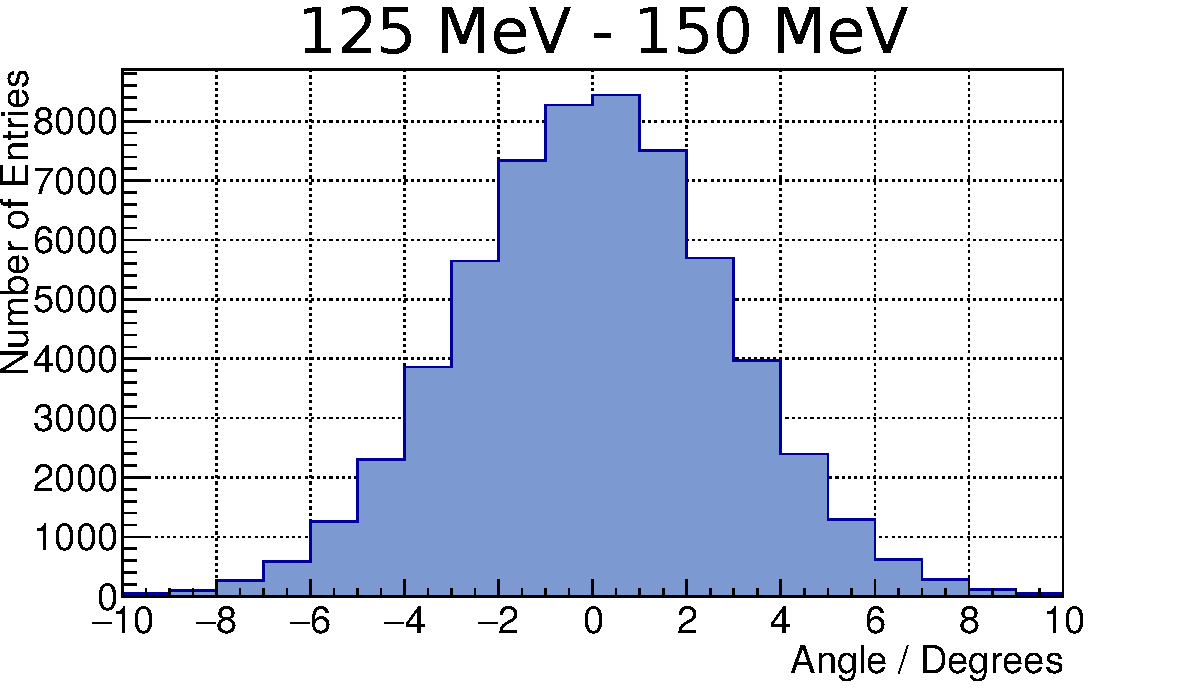
\includegraphics[width=0.35\textwidth]{Pictures/20170205DiffOeffZVertexUrsprung135MeV}	
	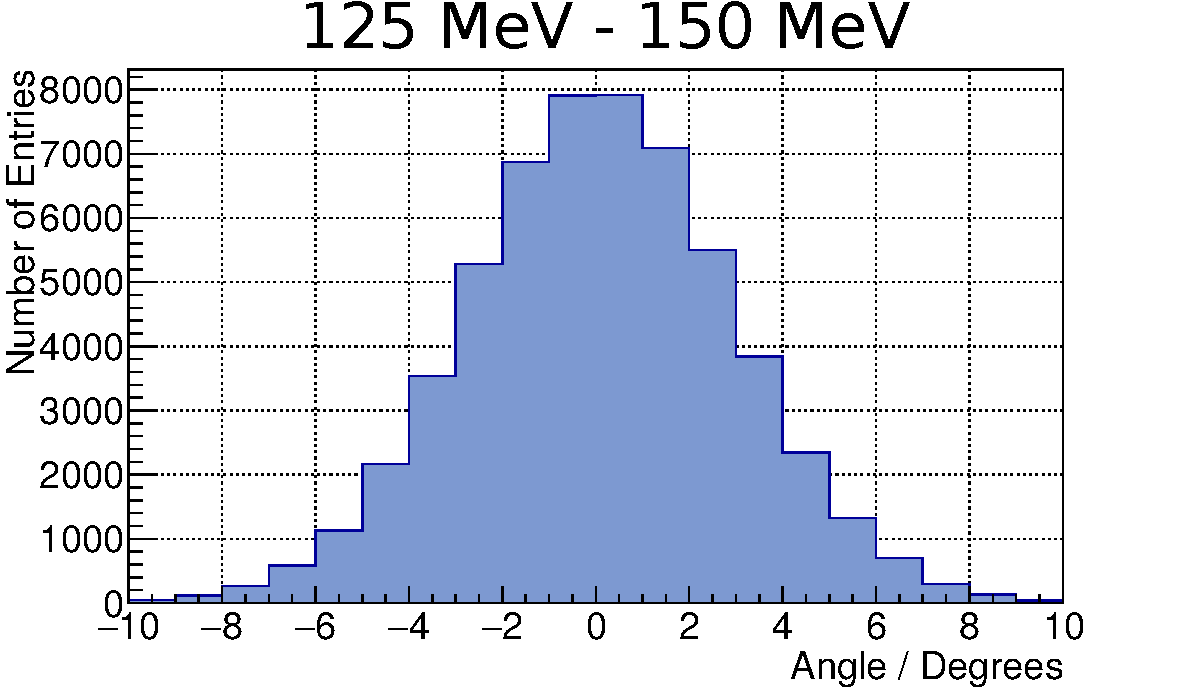
\includegraphics[width=0.35\textwidth]{Pictures/20170205DiffOeffZVertex+4_125MeV}	

	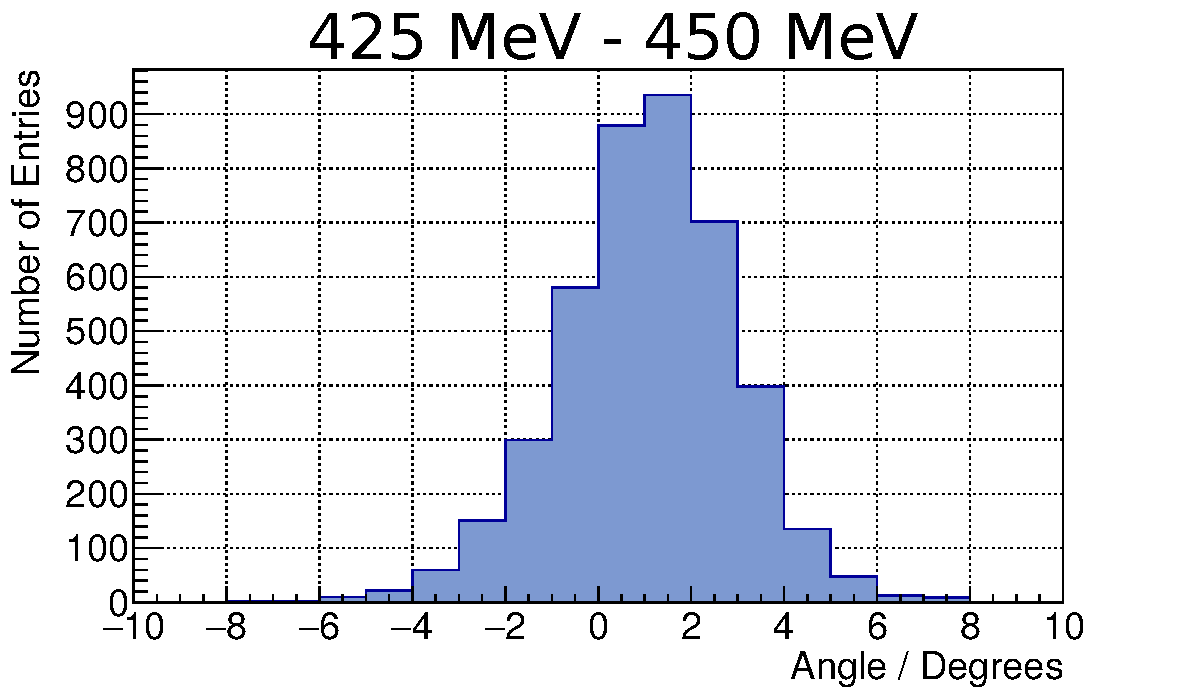
\includegraphics[width=0.35\textwidth]{Pictures/20170205DiffOeffZVertex-4_425MeV}
	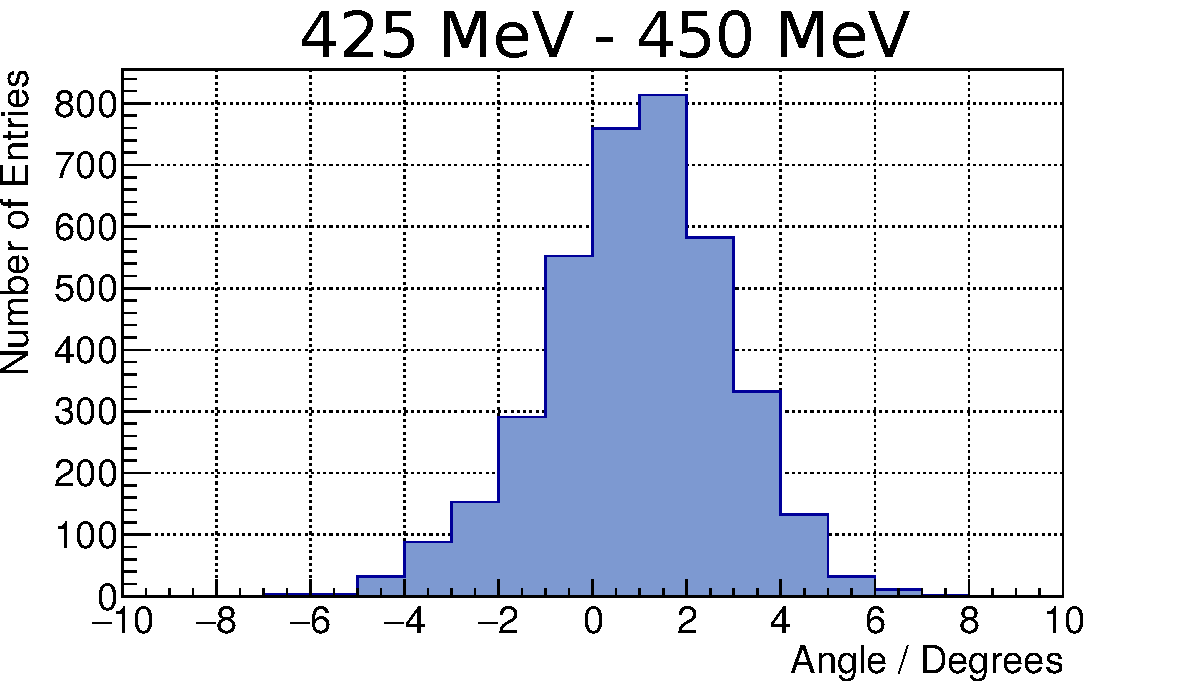
\includegraphics[width=0.35\textwidth]{Pictures/20170205DiffOeffZVertexUrsprung425MeV}
	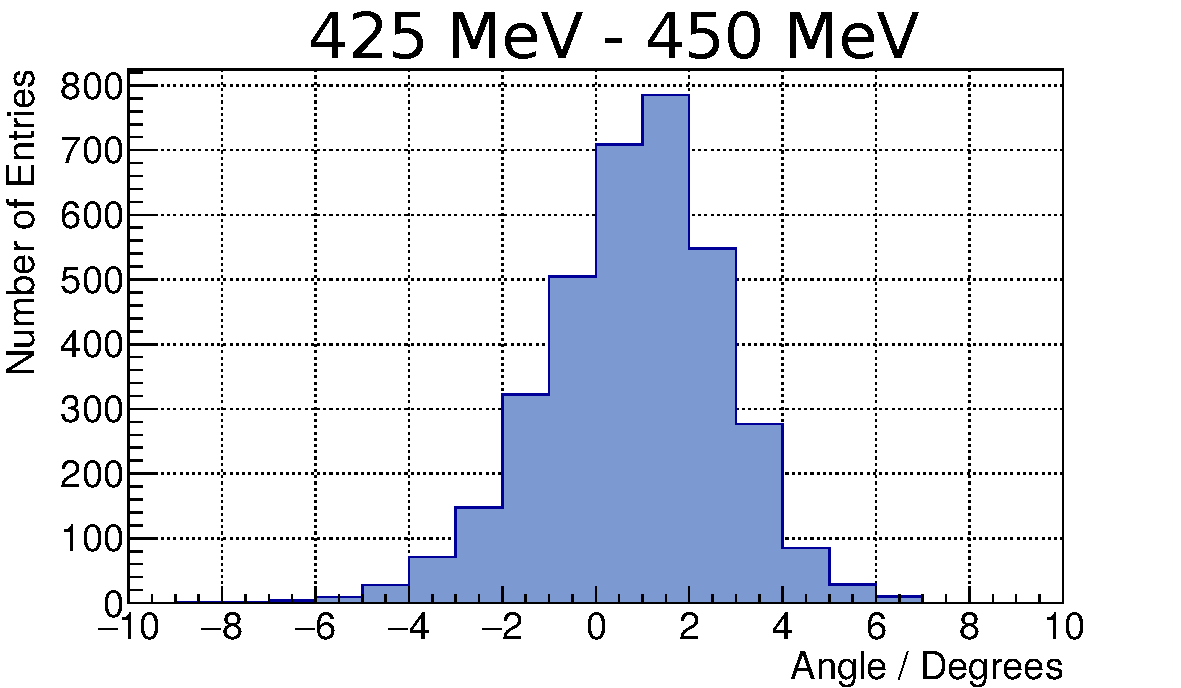
\includegraphics[width=0.35\textwidth]{Pictures/20170205DiffOeffZVertex+4_425MeV}	
	
\end{figure}
	
\end{frame}




\section{Further Results}
\begin{frame}
	\frametitle{Hot Crystals}
	\begin{itemize}
		\item Beamtime October 2014
		\item Photon energy between $0\,\text{MeV}$ and $100\,\text{MeV}$
	\end{itemize}
	\begin{figure}
		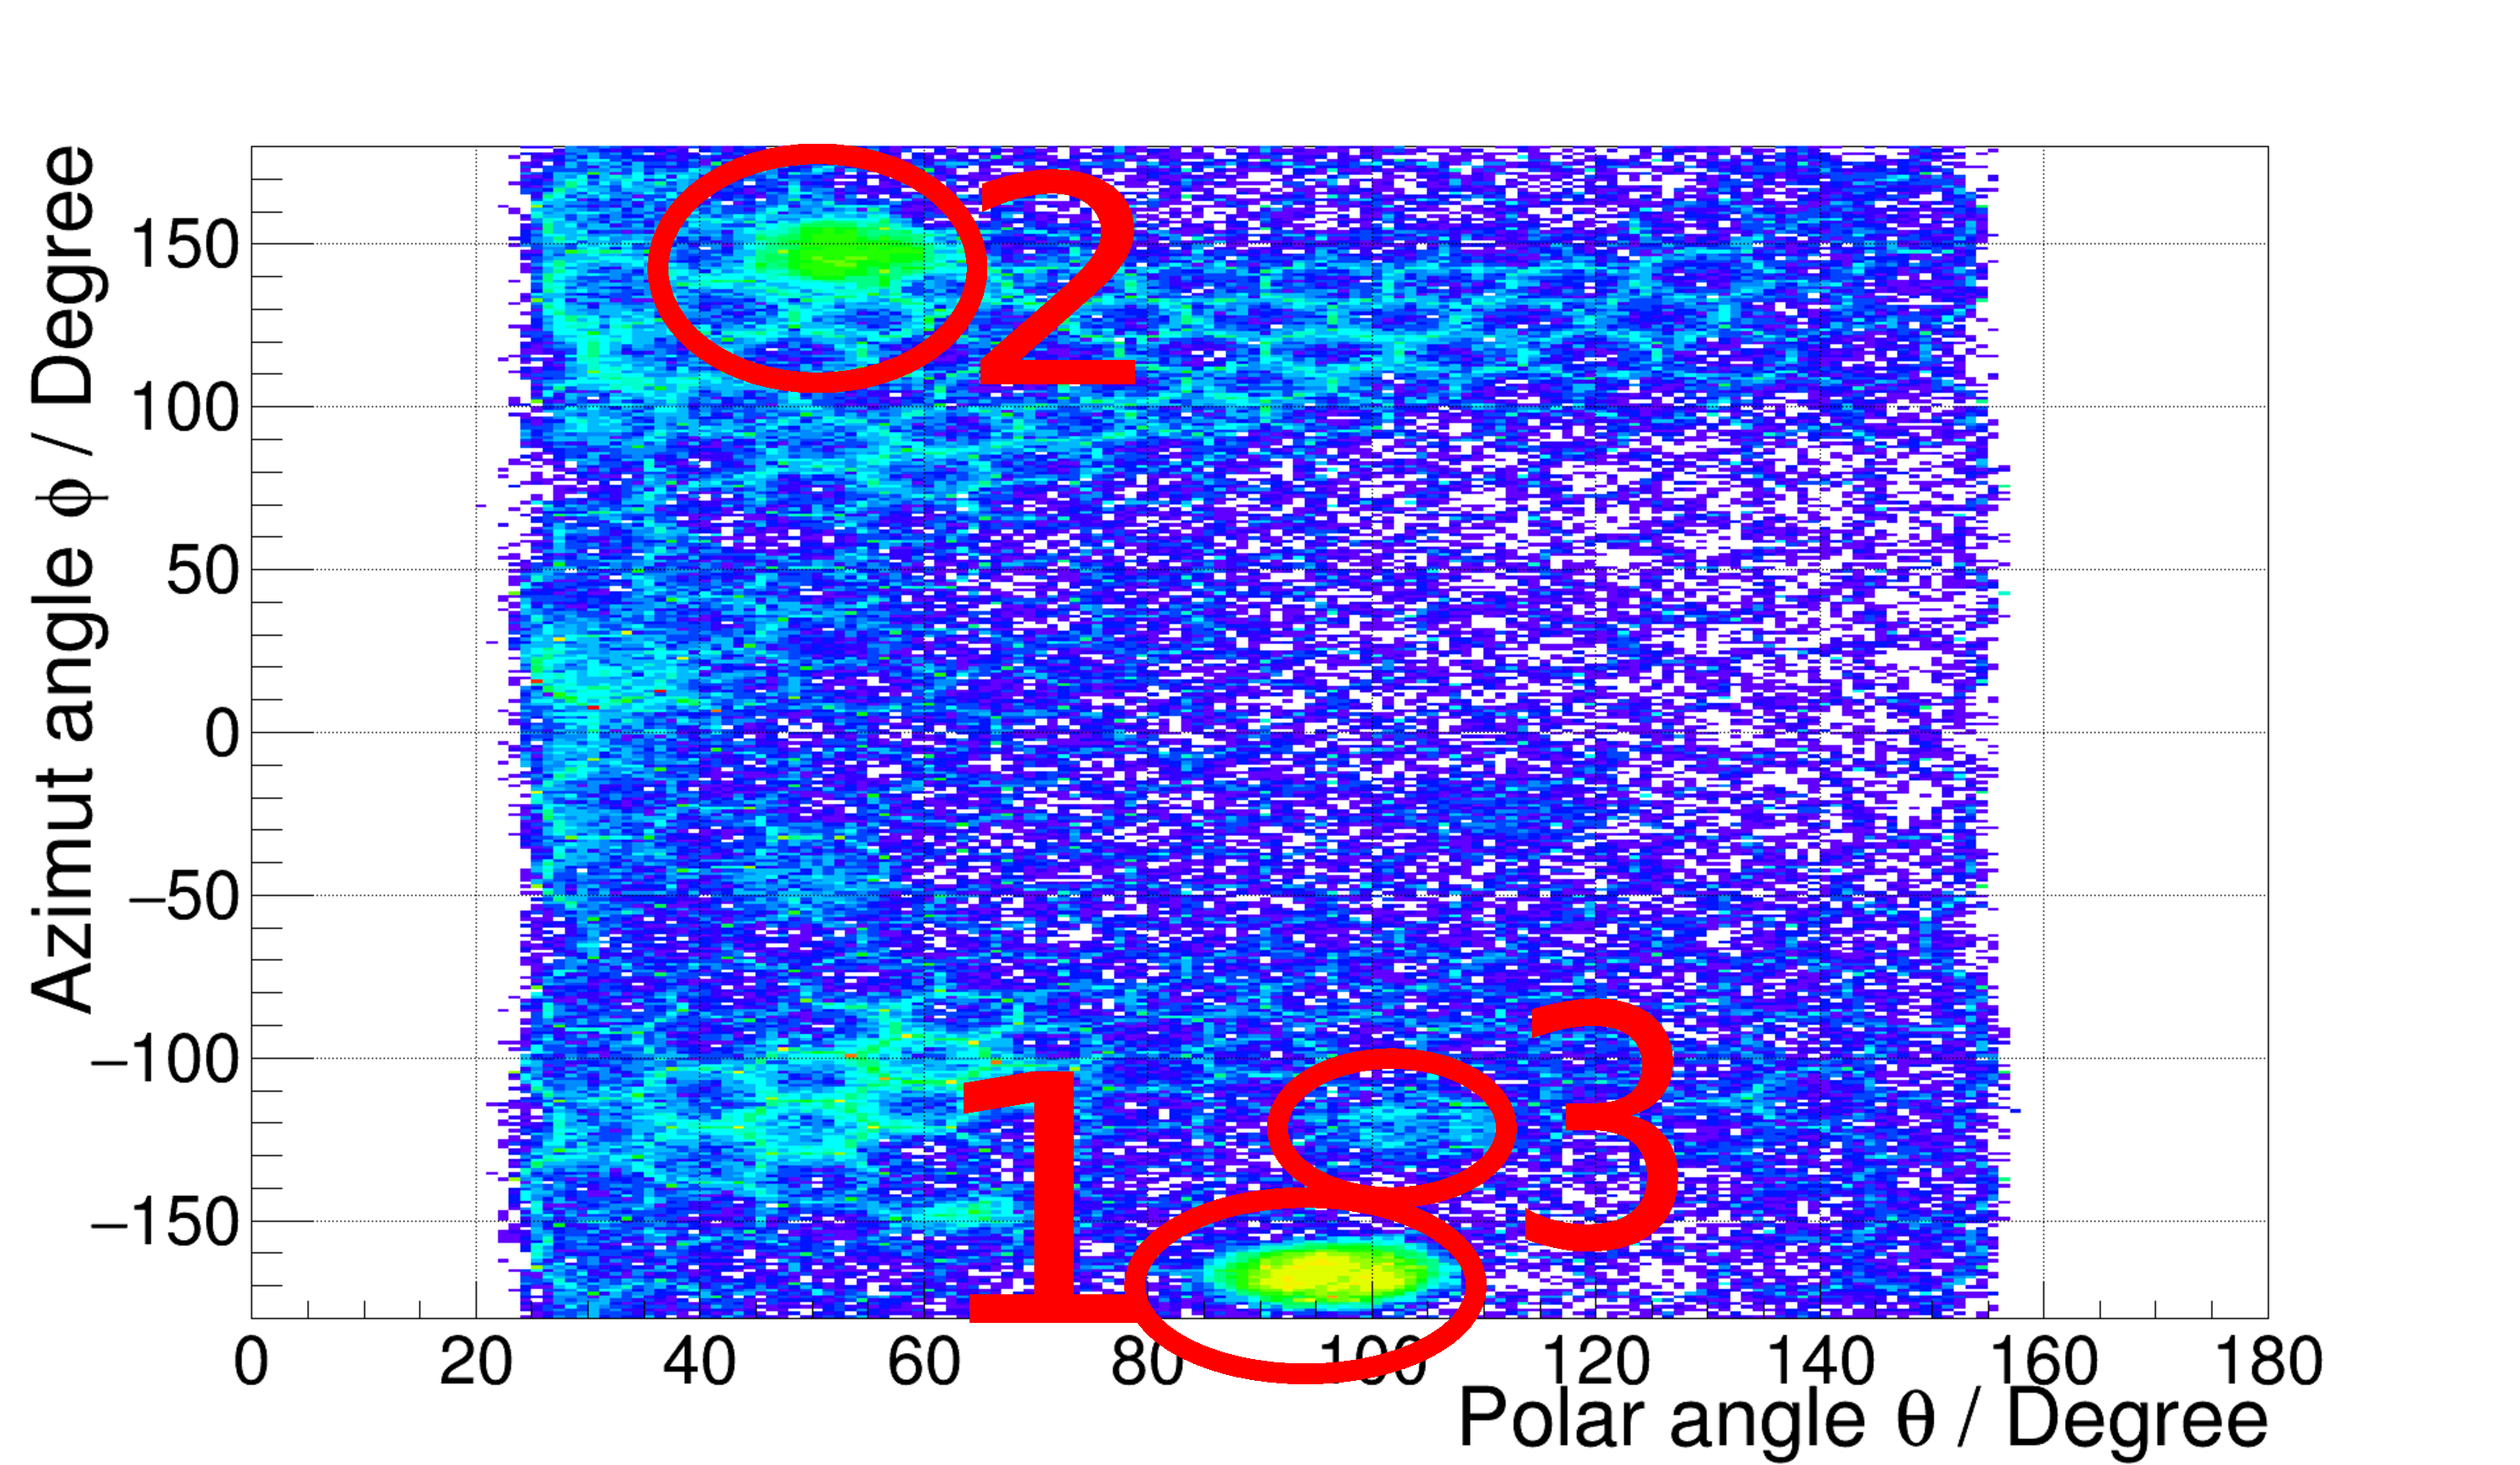
\includegraphics[width=0.50\textwidth]{Pictures/20172104StrahlzeitClusterSize0Marker}
		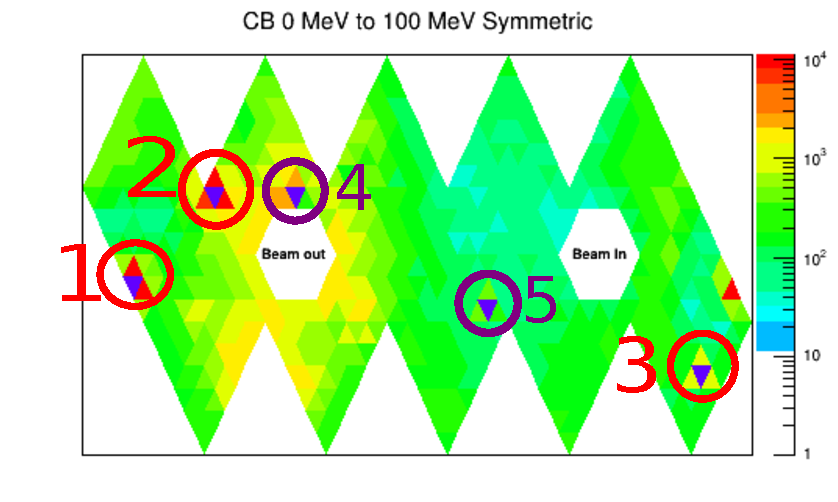
\includegraphics[width=0.50\textwidth]{Pictures/20172104StrahlzeitClusterSize0MarkerMap}
		
	\end{figure}
	\begin{table}
	
	\scalebox{0.7}{
	\begin{tabular}{lccccc}
		Number in the figures & 1 & 2 & 3 & 4 & 5 \\
		Element Number & 549 & 565 & 597 & 677 & 265 
		
	\end{tabular}}
	\end{table}
\end{frame}

\begin{frame}
	\frametitle{Hot Crystals and Clustersize $>$ 3}
	\begin{itemize}
		\item Beamtime October 2014
		\item Photon energy between $0\,\text{MeV}$ and $100\,\text{MeV}$
		\item Clustersize $>$ 3
	\end{itemize}

\begin{figure}
	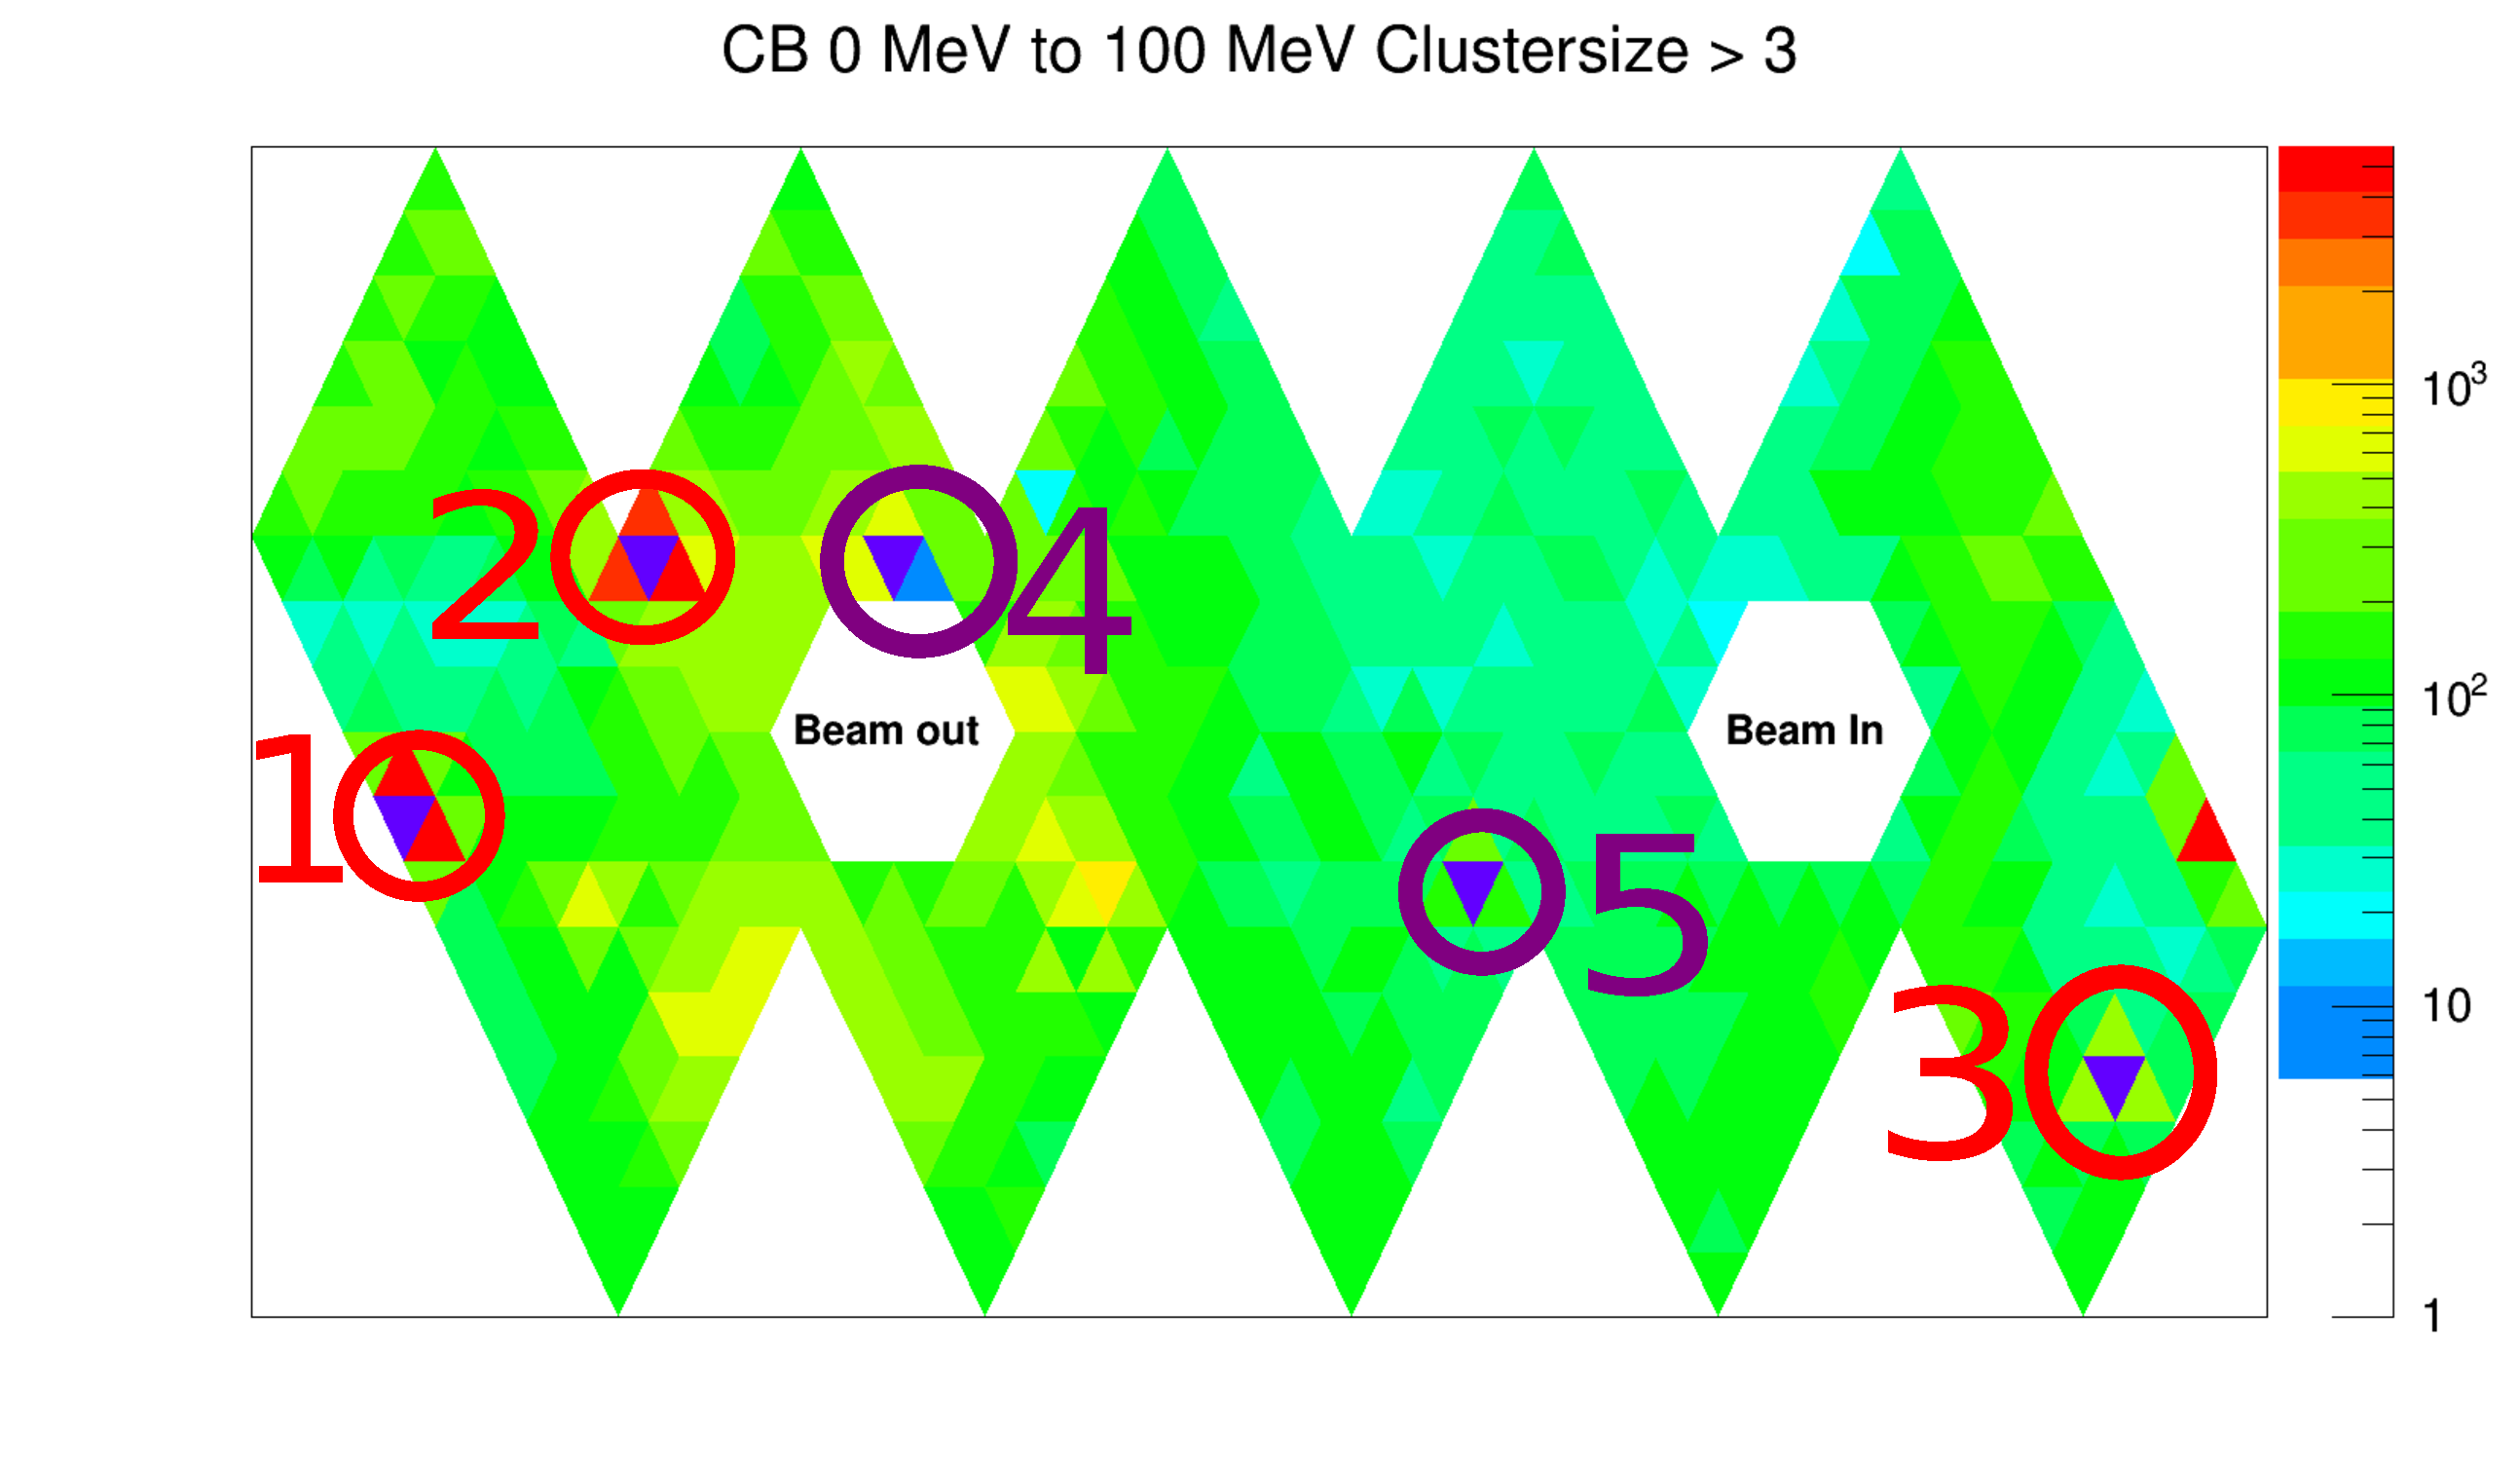
\includegraphics[width=0.75\textwidth]{Pictures/20172404Clustersize3Map100MeV}
	
\end{figure}


$\rightarrow$ Neighbors of some dead crystals appear hot for low energies
\end{frame}

\begin{frame}
	\frametitle{Hot Crystals for Higher Energies}
	\begin{itemize}
		\item Beamtime October 2014
		\item Photon energy between $300\,\text{MeV}$ and $400\,\text{MeV}$
	\end{itemize}
\begin{figure}
	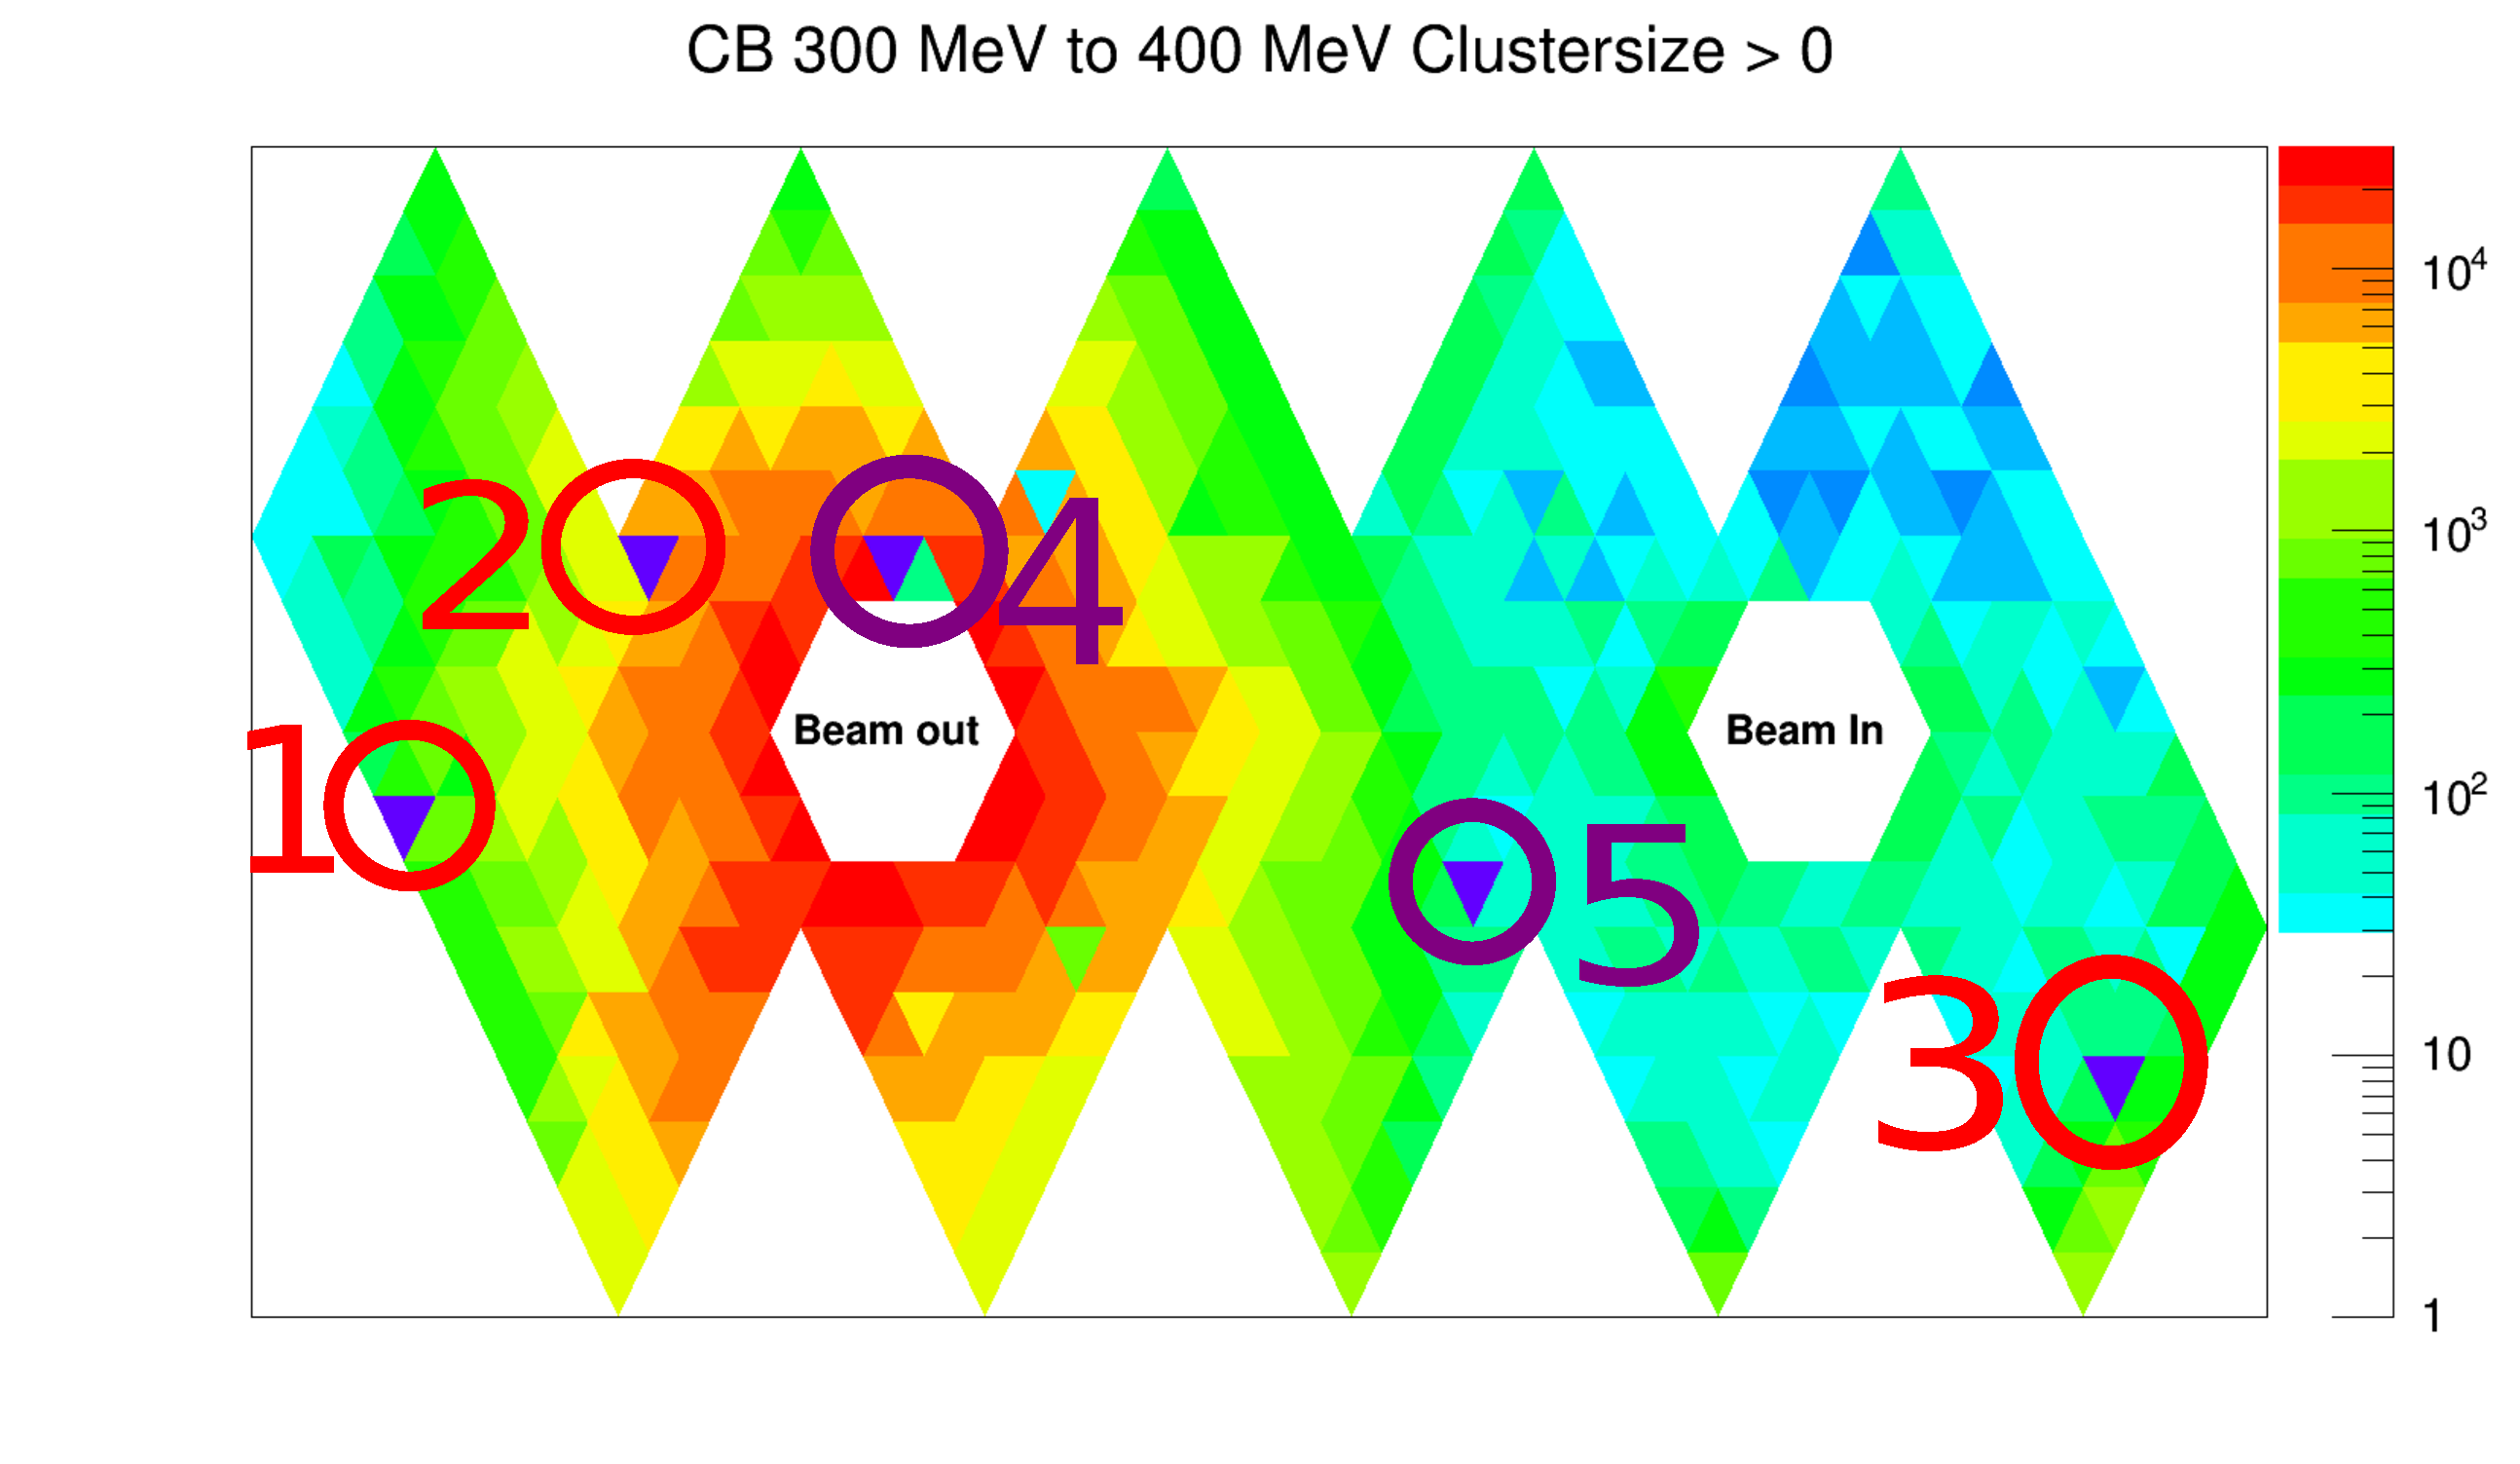
\includegraphics[width=0.75\textwidth]{Pictures/20172404Clustersize0Map400MeV}
	
\end{figure}
$\rightarrow$ \textit{Hot Neighbors} disappear at larger energies

\end{frame}

\begin{frame}
	\frametitle{Additional Dead Crystals}
	\begin{itemize}
		\item Beamtime October 2014
		\item Photon energy between $300\,\text{MeV}$ and $400\,\text{MeV}$
	\end{itemize}



	\begin{figure}
		\centering
		\begin{minipage}[t]{.6\textwidth}
			\centering
			\vspace{0pt}
			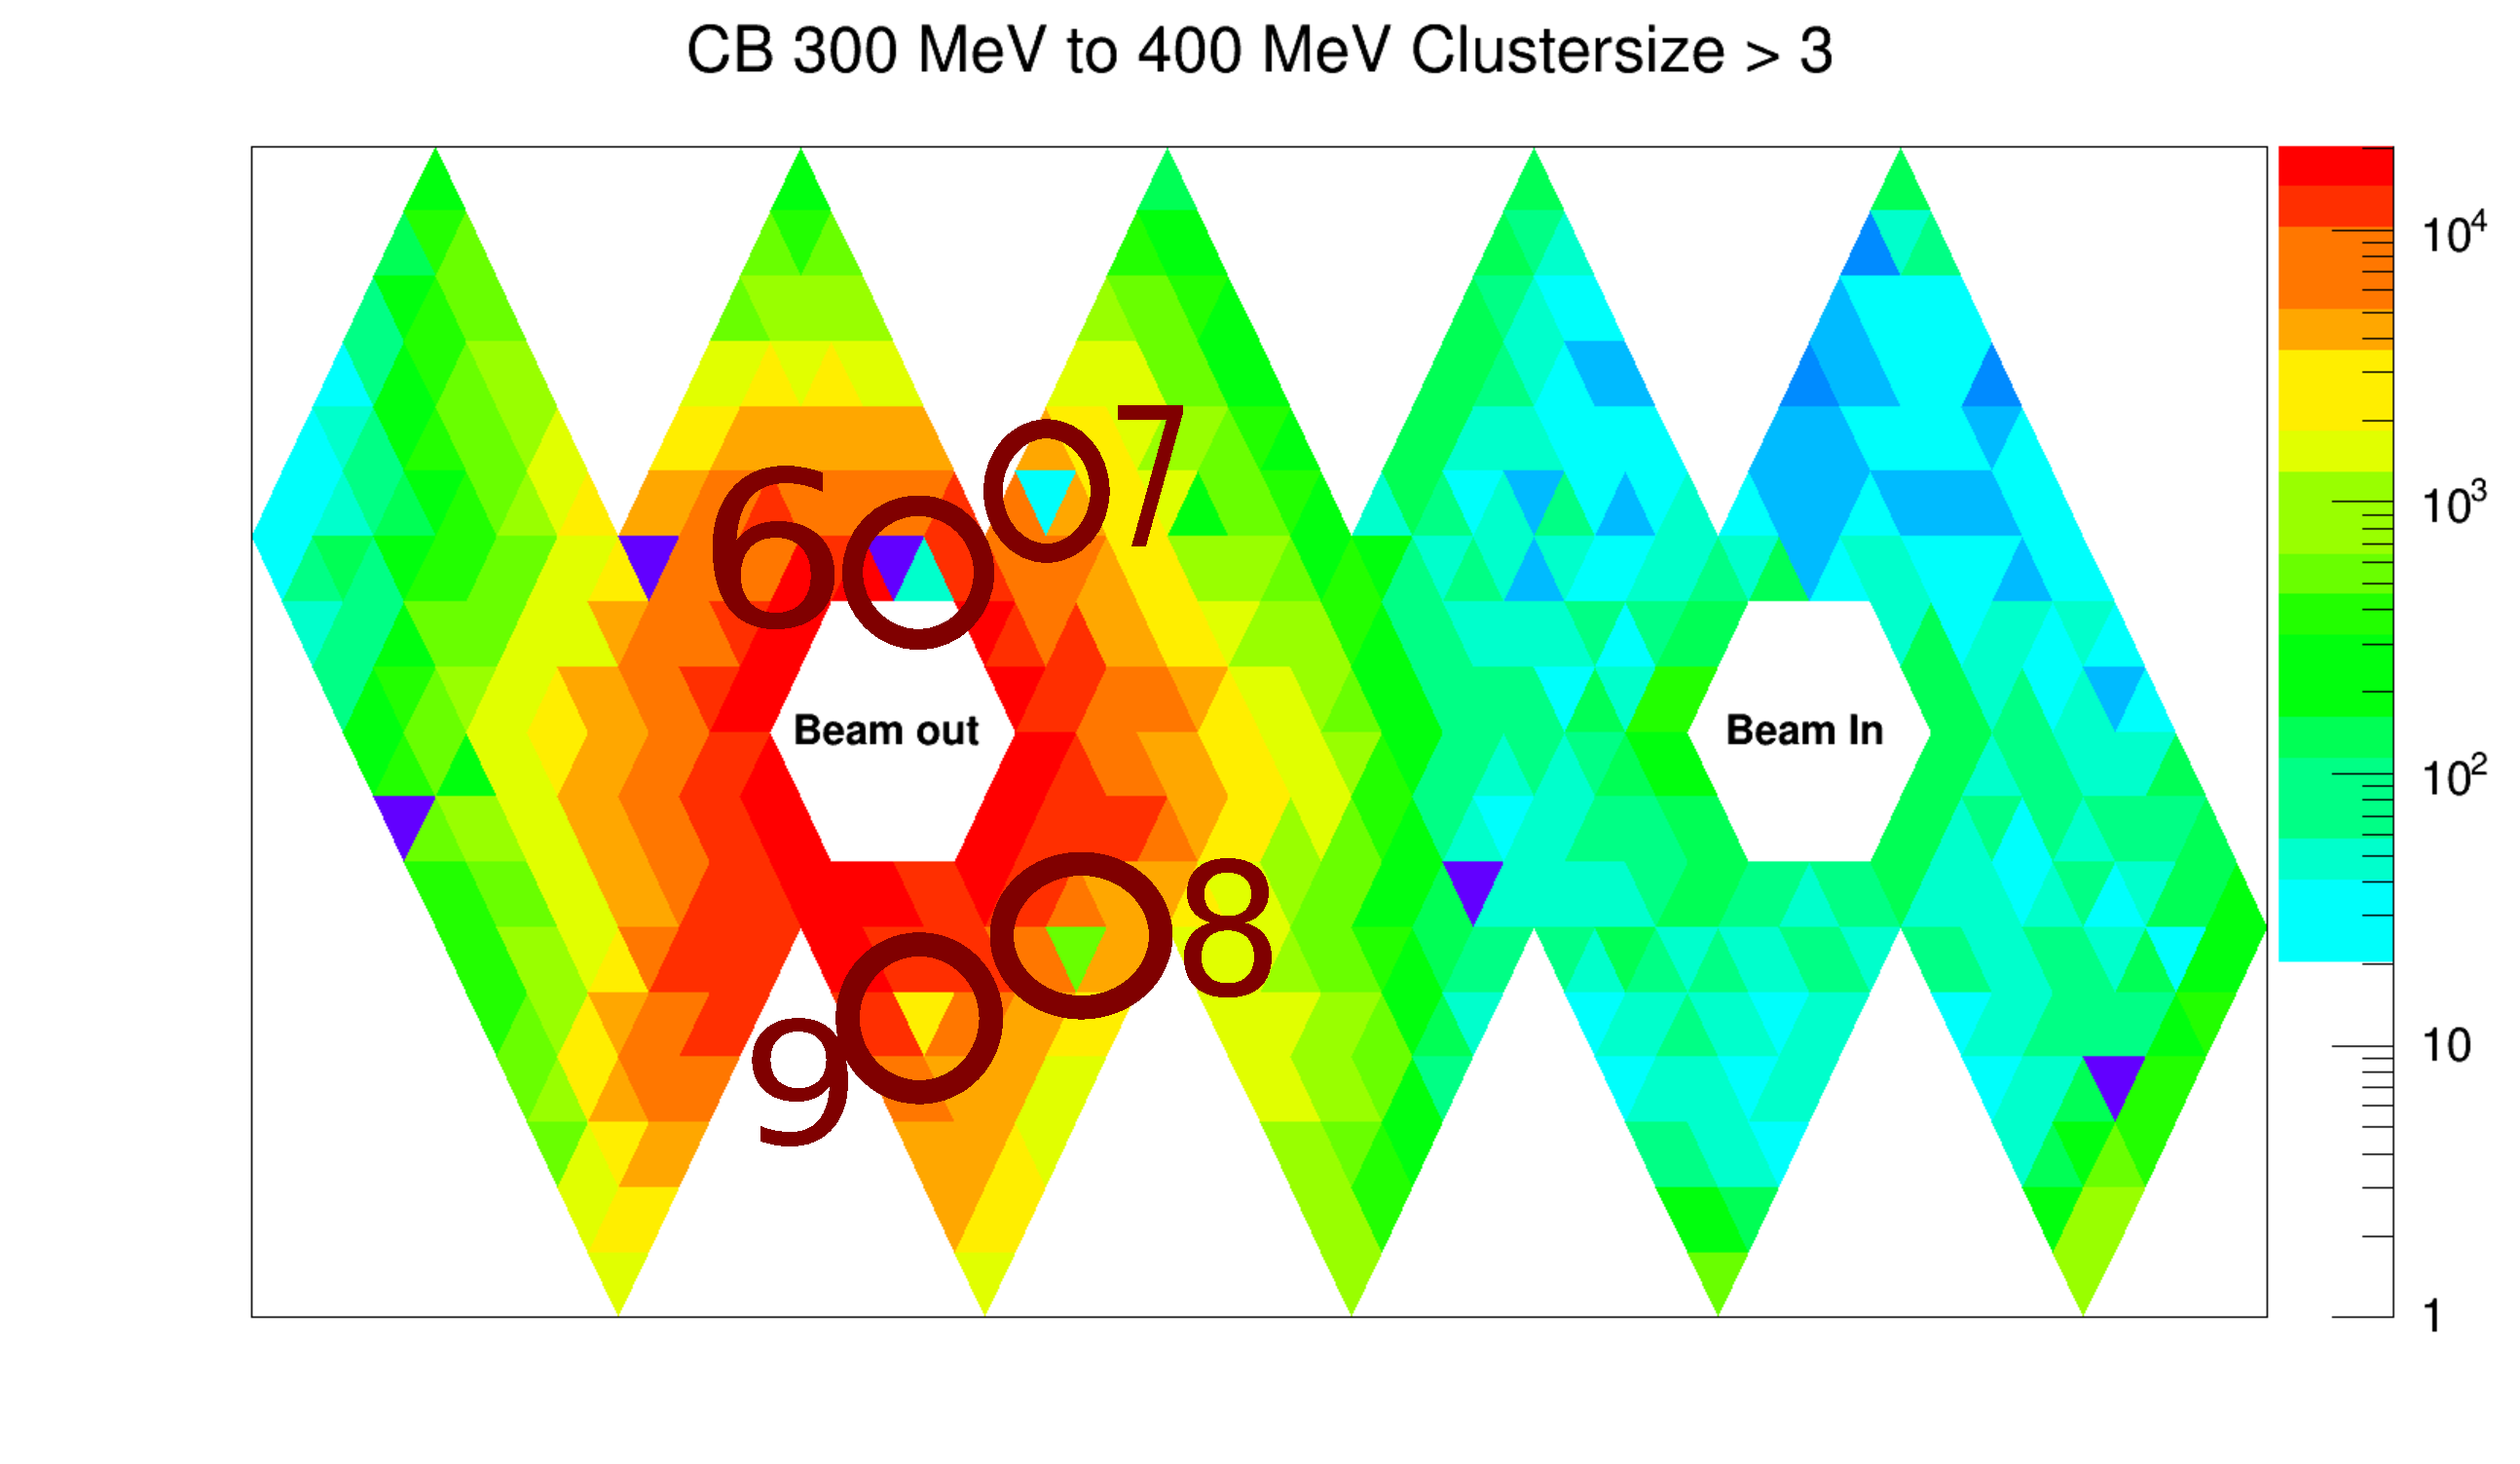
\includegraphics[width=\textwidth]{Pictures/20172504StrahlzeitMoreDead}
			
		\end{minipage}\hfill
		\begin{minipage}[t]{.4\textwidth}
			\centering
			\vspace{0pt}
			
		\scalebox{0.60}{
			\begin{tabular}{lcc}
				No. in Fig. & Element Number & No. of Hits \\
				
				\hline
				%\rowcolor{LightCyan}
				6& \textcolor{red}{678} &\textcolor{red}{48} \\
				
				& 677&0 \\
				
				& 676& 11808\\ 
				
				
				\hline
				7& \textcolor{red}{17} &\textcolor{red}{21} \\
				
				& 16 & 3311\\
				
				& 18& 7175 \\
				
				& 19& 3439 \\
				
				\hline
				
				8 & \textcolor{red}{125} &\textcolor{red}{513} \\
				
				
				& 122& 6613\\
				
				& 128 & 5307 \\
				
				& 126 & 4103 \\
				
				\hline
				
				9 & \textcolor{red}{89}& \textcolor{red}{2500}\\
				
				& 88& 8591\\
				
				&90&7975 \\
				
				&91&4652 \\
				
				
				
			\end{tabular}
		}	
		\end{minipage}
	\end{figure}
\end{frame}

\begin{frame}
	\frametitle{$\phi$-Distribution in the CB}
	\begin{itemize}
		\item Beamtime October 2014
		\item Photon energy between $200\,\text{MeV}$ and $225\,\text{MeV}$
		\item Weird bump
	\end{itemize}
	\begin{figure}
		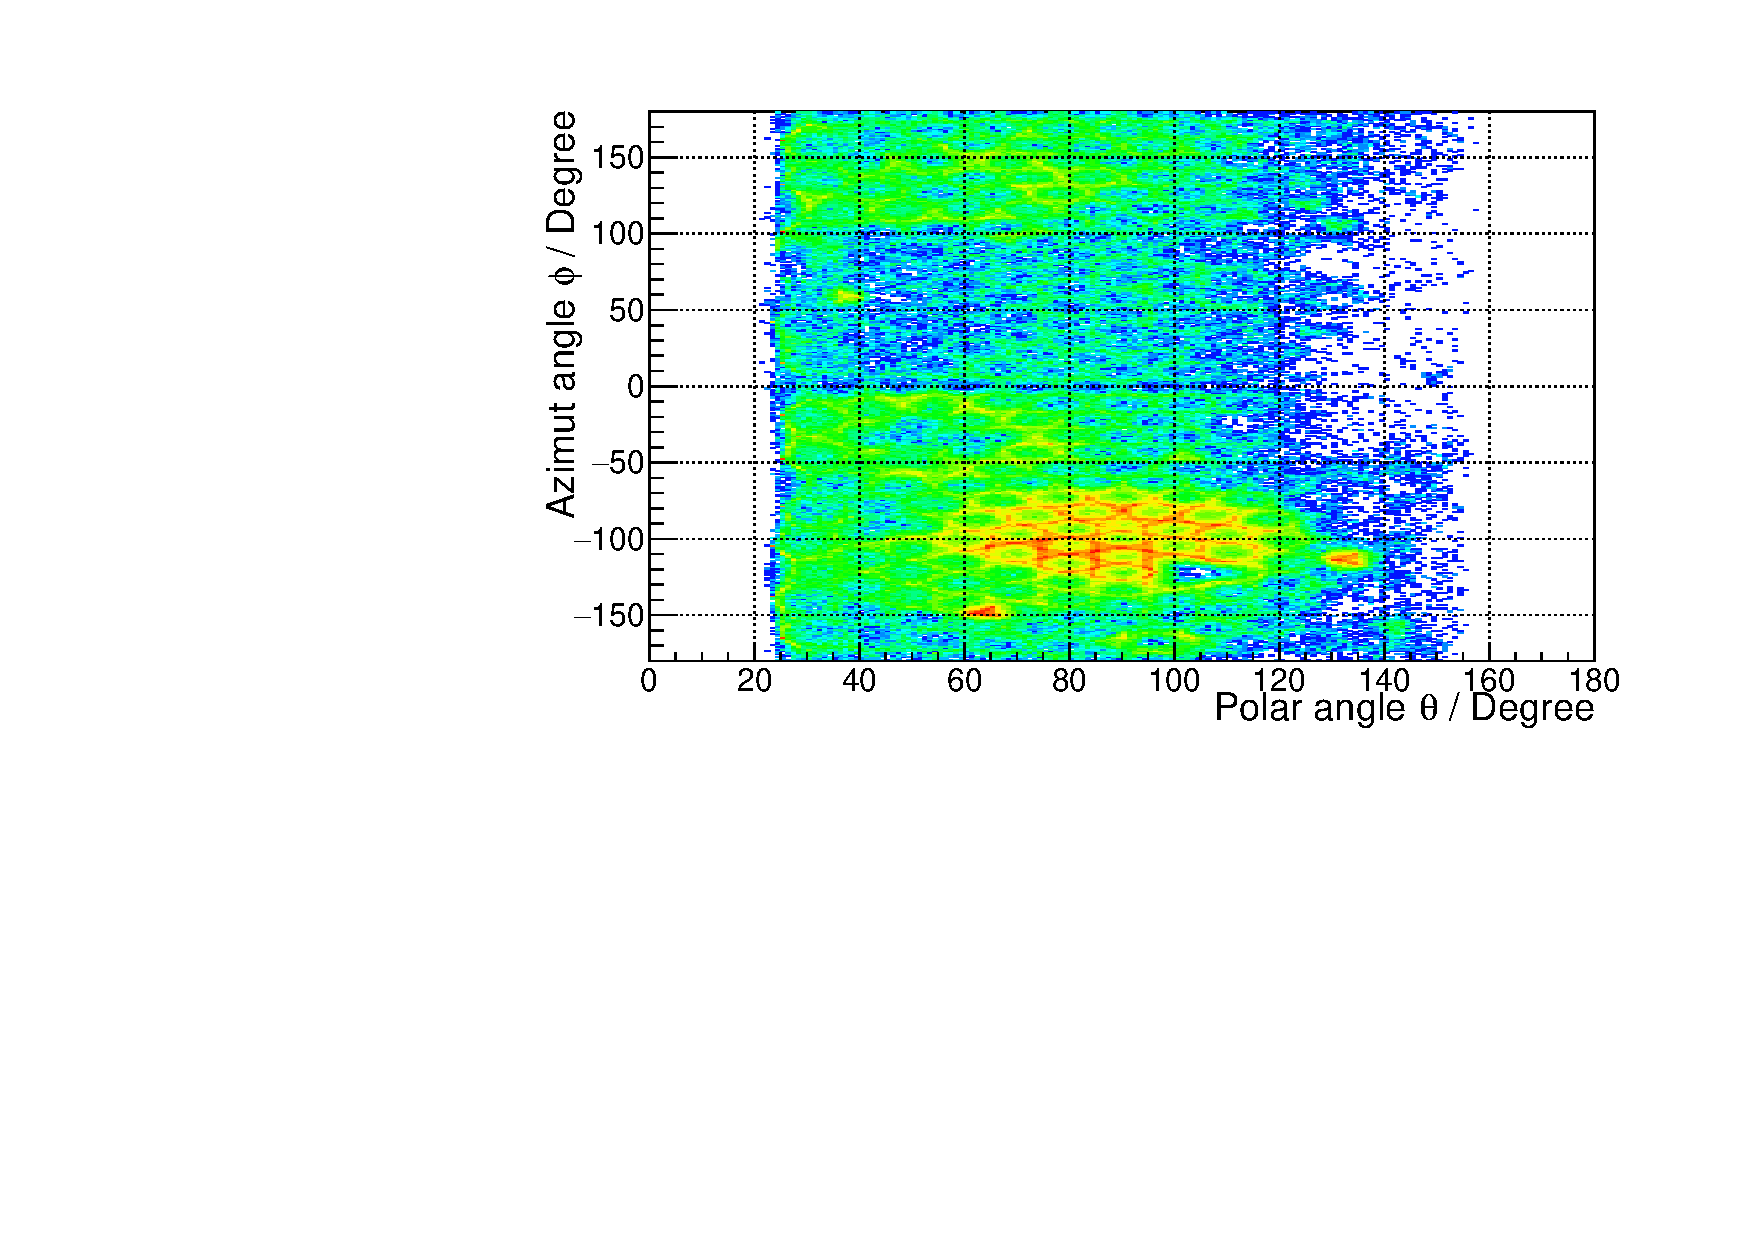
\includegraphics[width=0.75\textwidth]{Pictures/20172404ThetaPhi200MeVBeam}
		
	\end{figure}
\end{frame}


\section{Conclusion}
\begin{frame}
	\frametitle{Conclusion}
	\begin{itemize}
		\item There is a energy dependency in the detector
		\item The reconstructed opening angle is too big for high energies
		
		$\rightarrow$ wrong reconstruction of the photon impact position is probably the reason for the dependency (Clustering Algorithm) 
		\item The hardware of some PIDs has to be checked (too few or to many events)
		\item There is a strange $\phi$-distribution in the detector
		
		$\rightarrow$ reason for this has also to be determined
	\end{itemize}
\end{frame}
\section{Appendix}
\begin{frame}
	\frametitle{Appendix}
	
	\begin{figure}
		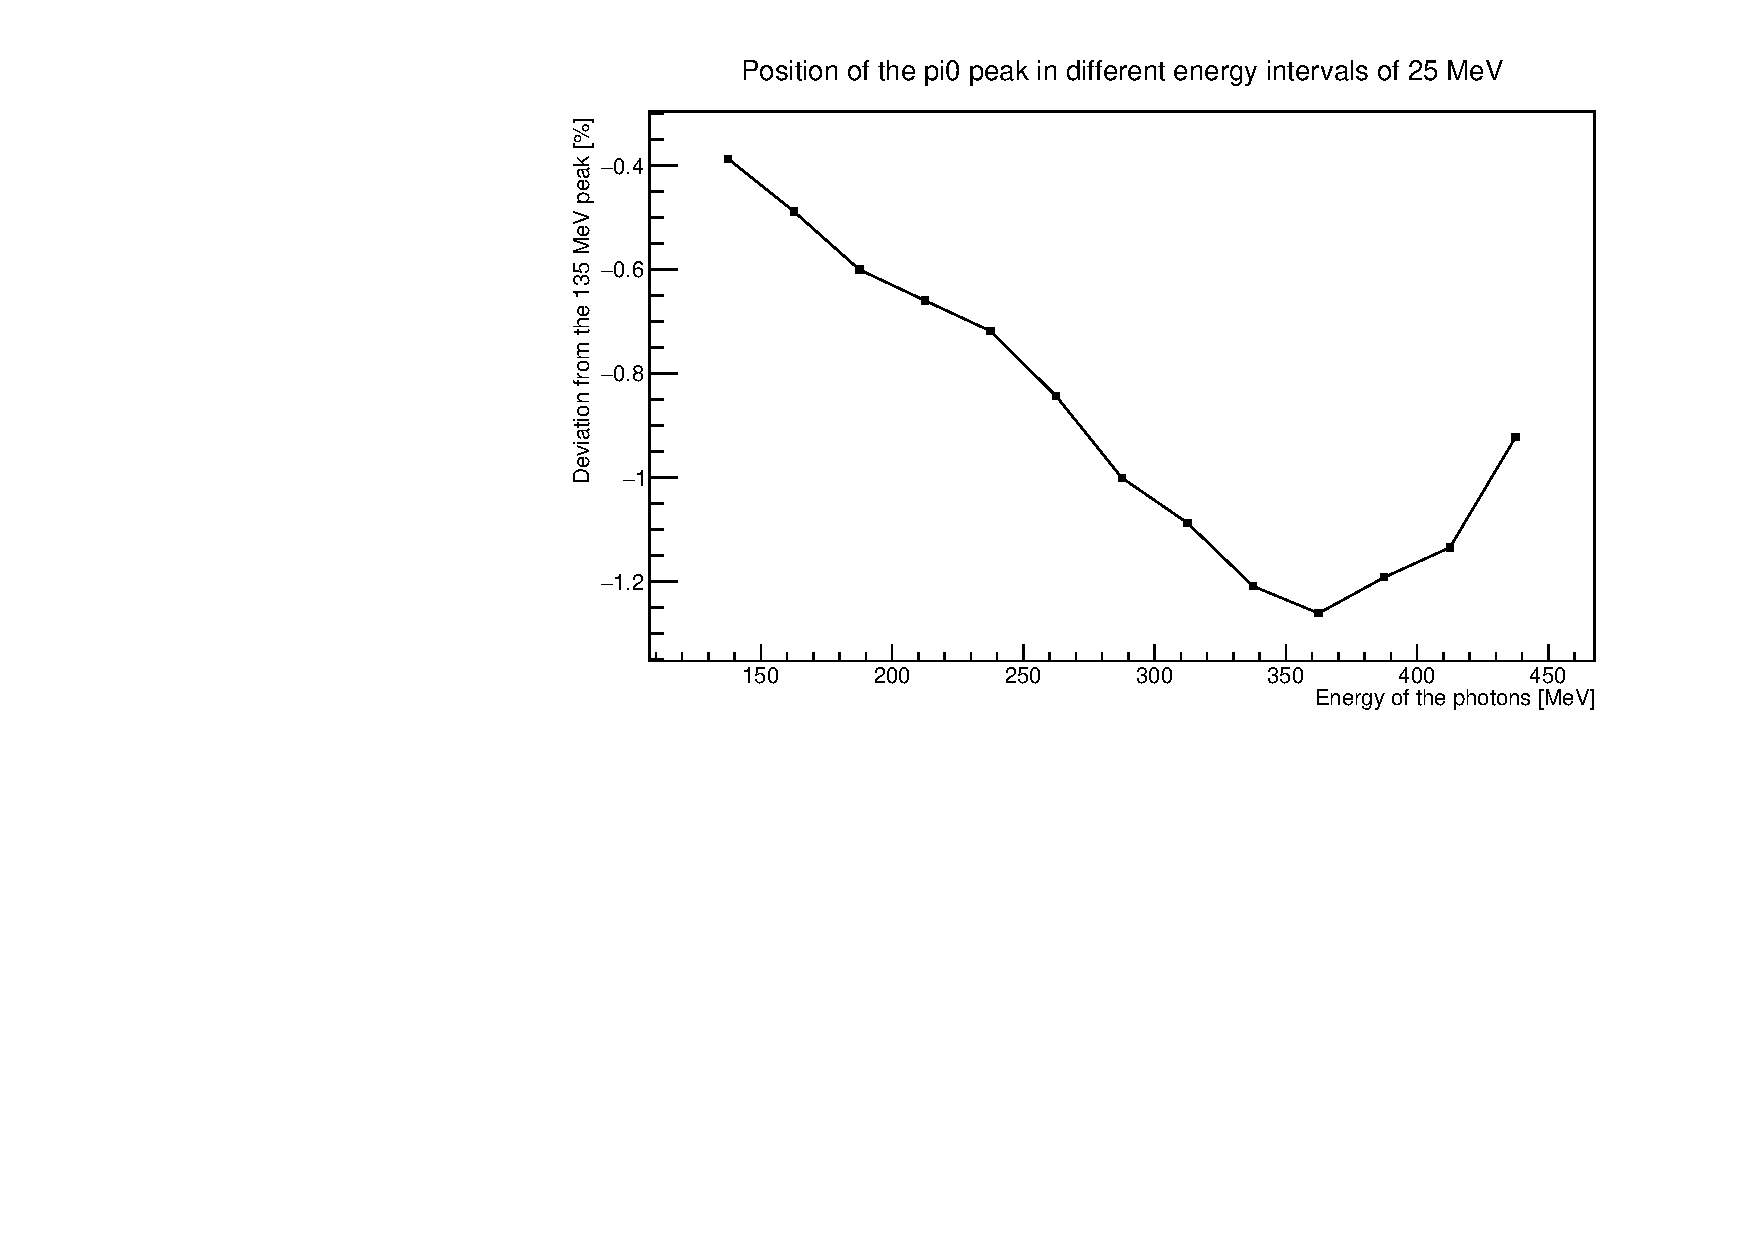
\includegraphics[width=0.5\textwidth]{Pictures/20170724RecETrueOAngle}
		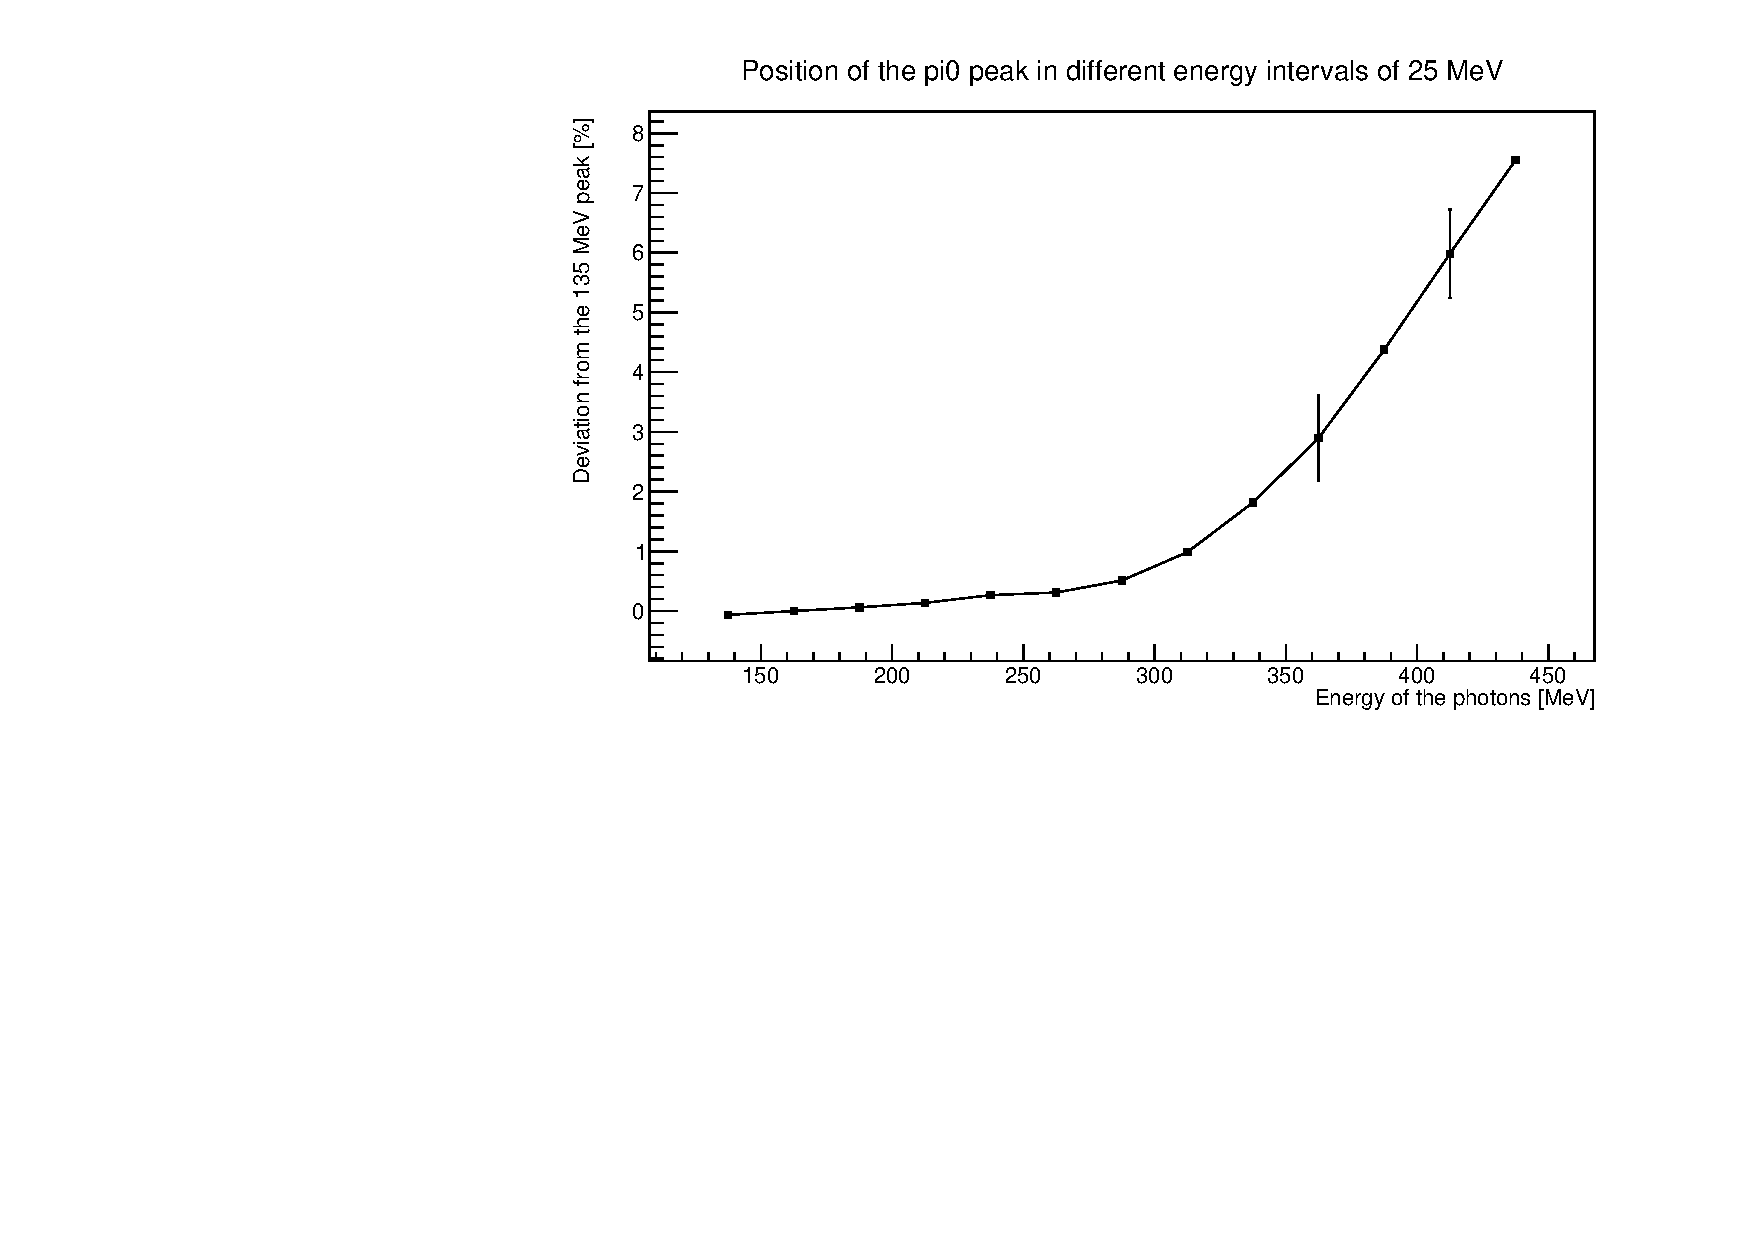
\includegraphics[width=0.5\textwidth]{Pictures/20170724TrueERecOAngle}
		\caption{Simulation:Left: Reconstructed energy and true opening angle. Right: True energy and reconstructed opening angle}
	\end{figure}
\end{frame}
\end{document} 